%% -----------------------------------------------------------------
%% This file uses UTF-8 encoding
%%
%% For compilation use following command:
%% latexmk -pdf -pvc -bibtex thesis
%%
%% -----------------------------------------------------------------
%%                                     _     _      
%%      _ __  _ __ ___  __ _ _ __ ___ | |__ | | ___ 
%%     | '_ \| '__/ _ \/ _` | '_ ` _ \| '_ \| |/ _ \
%%     | |_) | | |  __/ (_| | | | | | | |_) | |  __/
%%     | .__/|_|  \___|\__,_|_| |_| |_|_.__/|_|\___|
%%     |_|                                          
%%
%% -----------------------------------------------------------------

\documentclass{kithesis}

% Additional packages
\usepackage[main=english,slovak]{babel}
% For thesis written in English just change the order of languages:
% \usepackage[main=english,slovak]{babel}

\usepackage{listings}  % for source code
% Listings settings
% See for details: https://en.wikibooks.org/wiki/LaTeX/Source_Code_Listings
\usepackage{qtree}
\usepackage{tikz-qtree}
\usepackage{graphicx}
\usepackage{subcaption}

\lstset{
    basicstyle=\small\ttfamily,  % smaller typewriter font
    showstringspaces=false       % don't show spaces in string
}

% Location of file with bibliography resources
\addbibresource{chapters/bibliography.bib}

% Variables
%\thesisspec{figures/thesisspec.png} 

\title{Advanced prediction models for sales forecasting}{Advanced prediction models for sales forecasting}

\author[Bc.]{Aleš}{Jandera}
\supervisor{doc. Ing. Tomáš Škovránek, PhD.} %veduci prace
%\consultant{Donald E. Knuth} %konzultant
%\college{University of Žilina}{Žilinská univerzita} %univerzita
%\faculty{Faculty of Electrical Engineering and informatics}{Fakulta elektrotechniky a informatiky} %fakulta
%\department{Department of Computers and Informatics}{Katedra počítačov a informatiky} %katedra
%\departmentacr{DCI}{KPI} % skratka katedry
%\thesis{Master thesis}{Diplomová práca} %typ prace
\submissiondate{21}{4}{2023}
%\fieldofstudy{9.2.1 Informatika}
%\studyprogramme{Informatika}
%\city{Košice} %mesto
\keywords{Mathematic modeling, forecasting, linear prediction}{Matematické modelovanie, predpoved, lineárna predikcia}
%\declaration{som nepodvadzal}

\abstract{%
    % english 
	Sales forecasting can be divided into two main categories: short-term and long-term forecasting.
    Short-term forecasting is generally done on a weekly or monthly basis. Long-term forecasting is done on a quarterly or annual basis.
    There are many different methods that can be used for sales forecasting.
    The most common method is trend analysis. Trend analysis looks at past sales data to identify
    patterns and trends that can be used to predict future sales.
    Other methods include regression analysis and time series analysis.
    Advance prediction modeling is a type of long-term forecasting.
    It uses historical data and statistical techniques to predict future sales.
    Advance prediction modeling is often used by companies to make strategic decisions about inventory, pricing, and marketing.
}{%
    % slovak 
	Prognózy predaja možno rozdeliť do dvoch hlavných kategórií: krátkodobá a dlhodobá prognóza.
    Krátkodobé prognózy sa vo všeobecnosti vykonávajú týždenne alebo mesačne. Dlhodobé prognózy sa robia štvrťročne alebo ročne.
    Existuje mnoho rôznych metód, ktoré možno použiť na predpovedanie predaja.
    Najbežnejšou metódou je analýza trendov. Analýza trendov sa zameriava na údaje o minulých predajoch, aby identifikovala vzory a trendy,
    ktoré možno použiť na predpovedanie budúceho predaja. Ďalšie metódy zahŕňajú regresnú analýzu a analýzu časových radov.
    Predbežné predikčné modelovanie je typ dlhodobého predpovedania.
    Na predpovedanie budúceho predaja využíva historické údaje a štatistické techniky.
    Pokročilé predikčné modelovanie často používajú spoločnosti na strategické rozhodnutia o zásobách, cenách a marketingu.
}

\acknowledgment{Very strong thanks to whole teaching staff at the Institute of Control and Informatization of Production Processes for their patience,
leadership and knowledge which helped me to write this thesis.
I would like to express my deepest appreciation to my supervisor Tomas Skovranek for his time and advices.}

% if you want to work only on selected chapters
%\includeonly{chapters/analyza} %,chapters/synteza}

% Load acronyms
\input{acronyms}


%% -----------------------------------------------------------------
%%          _                                       _   
%%       __| | ___   ___ _   _ _ __ ___   ___ _ __ | |_ 
%%      / _` |/ _ \ / __| | | | '_ ` _ \ / _ \ '_ \| __|
%%     | (_| | (_) | (__| |_| | | | | | |  __/ | | | |_ 
%%      \__,_|\___/ \___|\__,_|_| |_| |_|\___|_| |_|\__|
%%                                                      
%% -----------------------------------------------------------------

\begin{document}
%% Title page, abstract, declaration etc.:
\frontmatter{}

%% List of code listings, if you are using package minted
%\listoflistings

%\pagenumbering{arabic}

%% Chapters
% !TEX root = ../thesis.tex

\chaptermark{Introduction}
\phantomsection
\addcontentsline{toc}{chapter}{Introduction}

\chapter*{Introduction}

Linear prediction~\cite{Vaidyanathan} is a method used in signal processing to predict future values of a time series based on past observations.
The technique is based on the assumption that the signal can be modeled as a linear combination of past values and a noise term.
Long-term linear prediction refers to the application of this method to predict values over a longer period of time, such as months or years.
It requires a greater amount of data and is more complex than short-term prediction, but can be useful in areas such as stock market forecasting and
weather prediction. The goal of this master thesis is to developing new algorithms and mathematical models to improve the accuracy of long-term predictions
in sales forecasting. Matlab \footnote{MATLAB is a fourth-generation programminglanguage and numerical analysis environment.
Uses for MATLAB include matrix calculations, developing and running algorithms, creating user interfaces (UI) and data visualization.}
livescript~\cite{livescript} will be used as development enviroment.

\section*{Task formulation}

Proposed a mathematical model and alghoritms for sales forcasting based on long-term prediction with improved Levinson - Durbin scheme 
which should have better performance and acuraccy than known linear prediction mechanism.

% !TEX root = ../thesis.tex

\chapter{Analytical part}\label{sec:analytical}

Linear prediction is~a statistical method used to predict future values based on historical data.
The Durbin-Levinson algorithm is~a~method for solving~the~linear prediction problem for autoregressive (AR)
models\footnote{Autoregressive (AR) models are time series models that describe~the~the~relationship between~the~current
value of~a~variable and its past values. In~an~autoregressive model, each observation is modeled as~a~linear
combination of past observations, with weights called AR coefficients. AR models are widely used in various fields
such as economics, engineering, and finance for modeling and forecasting time series data.~the~order of~the~AR model, denoted as "p", refers to~the~number of past values used to predict~the~current value. For example,~an~AR(1) model uses
only~the~previous observation to predict~the~current value, while~an~AR(2) model uses~the~previous two observations.},
which are models where~the~current output depends on previous outputs.~the~algorithm solves~the~linear prediction
problem by finding~the~coefficients of~the~AR model that minimize~the~prediction error.~the~resulting AR coefficients
can be used to make predictions about future values based on past observations. This method should be used with
using~the~pattern of linear relationship between~the~independent and dependent variables.
Here's~a~basic outline of~the~steps involved in using linear prediction to forecast sales data:\\
\begin{enumerate}
    \item Collect sales data: Gather~the~historical sales data for~the~product or service that we want to forecast.
    \item Plot~the~data: Plot~the~sales data over time to visually inspect~the~trend and identify any patterns.
    \item Choose~a~model: Select~an~appropriate linear model to represent~the~relationship between~the~independent and
    dependent variables in~the~data. For example, we might choose~a~simple linear regression model.
    \item Train~the~model: Train~the~selected model on~the~historical sales data using~a~method such as least squares
    regression.
    \item Make predictions: Use~the~trained model to make predictions on future sales data. We may want to generate
    predictions for several months or years in advance.
    \item Evaluate~the~model: Assess~the~accuracy of~the~predictions by comparing them to~the~actual sales data.
    Use metrics such as mean absolute error or root mean squared error to quantify~the~model's performance.
    \item Refine~the~model: If necessary, refine~the~model by adding additional independent variables or
    transforming~the~existing variables. Repeat~the~training and evaluation steps until we have~a~model that
    provides accurate forecasts.
\end{enumerate}
For shift calculation in longterm prediction can be used autocorrelation method, in this thesis neural network for
identification shift will be developed and similar mechanism for optimal order detection.

\section{Models used for sales data forecasting}\label{sec:models}
There are several mathematical models used for sales prediction, including Time series models~\ref{sec:timeseries} which are used to analyze and forecast sales data over time, such as seasonal patterns, trends, and fluctuations. Regression models~\ref{sec:regression} to use historical data to determine~the~relationship between sales and one or more independent variables, such as price, promotion, and advertising. Decision tree models~\ref{sec:trees} use~a~tree-like structure to make decisions based on~the~relationship between sales and multiple independent variables and machine learning models~\ref{sec:ml} to use algorithms such as neural networks and support vector machines to make predictions based on patterns in~the~data. \\
\\
The choice of mathematical model depends on~the~characteristics of~the~data,~the~desired level of accuracy, and the
computational resources available.
\\

\subsection{Time-series models}\label{sec:timeseries}
Time-series models are mathematical models used to analyze and forecast data that are collected over time~\cite{Cryer}.
These models are used to study and make predictions about~the~trends, patterns, and behavior of~the~data over time,
taking into account historical values and their relationship with~the~present. Time-series models are widely
used in areas such as economics, finance, and weather forecasting, among others.~the~models are based on various
statistical techniques, including ARIMA (AutoRegressive Integrated Moving Average), SARIMA (Seasonal ARIMA),
and exponential smoothing, among others.~the~goal of time-series modeling is to build~a~mathematical representation
of~the~underlying process that generates~the~time-series data, allowing for accurate prediction of future values.
Time-series models are statistical models used to analyze and make predictions about time-dependent data. They are
widely used in various fields, including finance, economics, engineering, and social sciences.
\\
Time-series models make use of past values of~a~variable to predict future values.
They assume that there is~a~pattern or trend in~the~data that can be used to forecast future behavior.
Some commonly used time-series models include:
\begin{itemize}
    \item Autoregressive Integrated Moving Average (ARIMA). This model is used to analyze and forecast stationary
    time-series data. It consists of three components: autoregression, differencing, and moving average.
    \item Seasonal Autoregressive Integrated Moving Average (SARIMA) is~an~extension of ARIMA
    that takes into account seasonal patterns in~the~data.
    \item Exponential Smoothing (ETS) is used to forecast time-series data that has~a~trend
    and/or seasonality. It uses~a~smoothing parameter to assign more or less weight to past observations
    based on their recency.
    \item Vector Autoregression (VAR) is used when there are multiple time-series variables
    that influence each other. It can be used to analyze~the~relationships between these variables and to make
    predictions about their future be   havior.
    \item These models are valuable tools for analyzing and predicting time-series data, but they require careful
    consideration of~the~specific characteristics of~the~data being analyzed and~the~appropriate model to use.
\end{itemize}

\subsection{Regression models}\label{sec:regression}
Regression models are~a~type of statistical models used to examine~the~relationship between~a~dependent variable
and one or more independent variables~\cite{Fahrmeir}.
The goal of regression analysis is to model~the~relationship between these variables and make predictions about
the dependent variable based on~the~values of~the~independent variables. Regression models are widely used in many
fields, including economics, finance, marketing, and social sciences, to make predictions and understand the
relationship between variables. There are several types of regression models, including:
\begin{itemize}
    \item Linear regression is~a~simple regression model where~the~relationship between~the~dependent and independent
    variables is modeled using~a~linear equation.
    \item Logistic regression is used for binary classification problems where~the~dependent variable is binary and~the~goal is to model~the~relationship between~the~independent variables and~the~probability of~the~dependent
    variable being either 0 or 1.
    \item Multiple regression is used when there are multiple independent variables and~the~goal is to model the
    relationship between all of these variables and~the~dependent variable.
    \item Polynomial regression is used when~the~relationship between~the~dependent and independent variables
    is non-linear and can be modeled using~a~polynomial equation.
\end{itemize}

The choice of regression model depends on~the~nature of~the~data and~the~research question being asked.

\subsection{Decision tree models}\label{sec:trees}
Decision tree models are~a~type of machine learning models used for both regression and classification
tasks~\cite{Kotsiantis}. They are tree-like structures that make predictions by breaking down~a~dataset into
smaller and smaller subsets, based on~the~values of~the~input variables. At each internal node of~the~tree,
a decision rule is used to split~the~data based on~the~value of~a~feature, and~the~process continues until the
data are separated into homogeneous groups, or leaves.
The predictions are then made based on~the~average or majority class in each leaf node. On figure~\ref{fig:example_tree} we can see example schema how~the~decision tree works.\\
\begin{figure}
    \centering
    \begin{tikzpicture}
        \Tree [.S        [.NP            [.Det the ]
                [.N cat ]
            ]
            [.VP            [.V chased ]
                [.NP                [.Det the ]
                    [.N mouse ]
                ]
            ]
        ]
    \end{tikzpicture}   
    \caption{Example of decission tree flow.}\label{fig:example_tree}
\end{figure}
\\
Decision trees have several advantages, including ease of interpretability, handling of non-linear relationships,
and ability to handle both categorical and numerical data. Some examples of decision tree algorithms are CART
(Classification and Regression Tree) and Random Forest.
\\
The decision tree model is trained using~a~dataset, and~the~tree structure is built using~a~greedy algorithm
that seeks to maximize~the~reduction in impurity of~the~target variable at each split.~the~model can then be used
to make predictions on new data by following~the~decision rules in~the~tree.
\subsection{Machine learning models}\label{sec:ml}
Machine learning models are~a~subset of artificial intelligence that allows computers to learn and make
predictions or decisions without being explicitly programmed. Machine learning models are based on algorithms
that use statistical methods to find patterns in data and make predictions about new, unseen data.
\\
There are several types of machine learning models, including \textbf{Supervised learning} where~the~model is trained on labeled data, with~the~goal of learning~the~relationship between~the~input features and~the~target variable, and making predictions about~the~target variable for new, unseen data.
\textbf{Unsupervised learning} where~the~model is trained on unlabeled data, with~the~goal of finding patterns or structure in~the~data, such as clustering or dimensionality reduction. \textbf{Reinforcement learning} where~the~model learns by receiving rewards or penalties for its actions in~an~environment, with~the~goal of maximizing~the~reward over time. \textbf{Deep learning} a~subset of machine learning that uses artificial neural networks with multiple hidden layers to model complex relationships in~the~data. 

The choice of machine learning model depends on~the~problem being solved and~the~type of data being used. Machine
learning models have been applied to~a~wide range of tasks, including image and speech recognition, natural language
processing, and predictive modeling. Advances in machine learning (ML), faster processors and~the~availability of
digitized healthcare data have contributed to~a~growing number of papers describing ML applications in healthcare~\cite{Chen}.\\
\\
\textbf{K-Nearest Neighbors (KNN)} \label{sec:knn}\\
Machine learning algorithms, K-Nearest Neighbors (KNN), is~a~type of artificial intelligence that allows
computers to learn and make decisions based on data. KNN is~a~simple yet effective algorithm used for
classification and regression tasks in supervised learning.\\
\\
KNN is~a~non-parametric algorithm, which means it doesn't make any assumptions about~the~underlying
distribution of~the~data. Instead, it uses~the~similarity between data points to classify or predict~the~target
variable.~the~algorithm works by finding~the~k-nearest neighbors to~a~new data point and then assigning~the~class
label of~the~majority of those neighbors to~the~new data point.\\
\\
For example, if we have~a~dataset of images with labels indicating whether each image contains~a~cat or~a~dog,
we can use KNN to classify~a~new image by finding~the~k-nearest neighbors to~the~new image and assigning the
label of~the~majority of those neighbors to~the~new image.\\
\\
KNN is~a~relatively simple algorithm, but it can be very effective when applied to~the~right problems.
It is particularly useful in cases where~the~decision boundary is nonlinear or where there is no clear
separation between classes. However, KNN can be computationally expensive when working with large datasets, and
it may not perform well in high-dimensional spaces.


\section{Neural networks} \label{sec:nn}
A neural network is~a~type of machine learning algorithm inspired by~the~structure and function of biological neurons
in~the~human brain. It is composed of interconnected nodes, called neurons, that are organized into layers.~the~input
layer receives raw data, such as images or text, and passes it on to~the~hidden layers, which perform calculations and
apply weights to~the~input data to create~a~prediction. Finally,~the~output layer produces~the~final prediction
or classification.\\
\\
As we can see on image \ref{fig:perceptron} each input $X_n$ should be properly weighted by~a~certain weight $W_n$ before
all~the~signals enter~the~summation stage. Afterwards,~the~weighted summation is forwarded into~the~activation unit
producing~the~neuron’s output signal.
\begin{center}
    \begin{figure}[!ht]
        \centering
        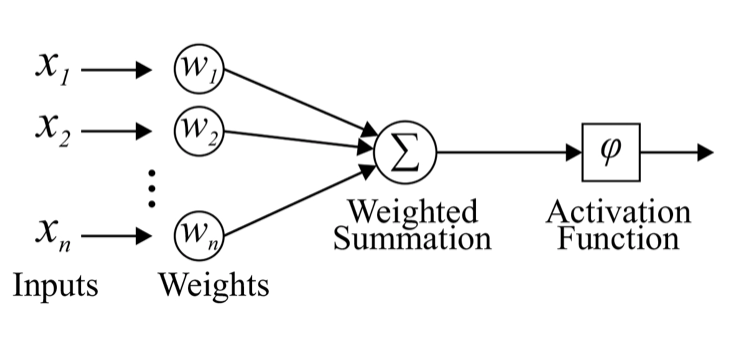
\includegraphics[width=1\textwidth]{figures/nn}
        \caption{Perceptron preview. \cite{Mourgias-Alexandris:19}}
        \label{fig:perceptron}
    \end{figure}
\end{center}
Neural networks are trained on large datasets using~a~process called backpropagation, which adjusts~the~weights and
biases of~the~neurons to minimize~the~error between~the~predicted output and~the~actual output. Once~a~neural network
has been trained, it can be used to make predictions on new data.\\
\\
A neuron is~a~basic building block of~a~neural network, also known as~an~artificial neuron or~a~perceptron.
It is modeled after~the~biological neuron in~the~human brain, which receives input signals from other neurons,
processes them, and sends output signals to other neurons.\\
\\
In~a~neural network,~a~neuron receives input from other neurons or directly from~the~input data, applies~a~mathematical
function to~the~input, and produces~an~output that is sent to other neurons in~the~network.~the~input to~a~neuron is
usually~a~vector of numbers, and each input is multiplied by~a~corresponding weight.~the~neuron then sums up the
weighted inputs, adds~a~bias term, and applies~an~activation function to~the~result.\\
\\
The purpose of~the~activation function is to introduce nonlinearity into~the~neuron, which allows~the~neural network
to learn complex patterns and relationships in~the~data. There are several different types of activation functions
that can be used, such as~the~sigmoid function, ReLU (Rectified Linear Unit) function, and tanh (hyperbolic tangent)
function.\\
\\
The output of~a~neuron is typically fed into other neurons in~the~next layer of~the~neural network.~the~weights and
biases of~the~neurons are adjusted during~the~training process using~a~technique called backpropagation, which involves
computing~the~gradient of~the~error with respect to~the~weights and updating them using~an~optimization algorithm such
as stochastic gradient descent.\\
Overall,~the~neurons in~a~neural network work together to learn patterns and relationships in~the~input data and produce
output that can be used for~a~variety of tasks, such as classification, regression, and prediction.\\
Neural networks have been successfully applied in~a~wide range of fields, including image and speech recognition, natural language processing, and autonomous vehicles, among others.
Neural networks can be broadly classified into~the~following types:\\
\\
\textbf{Feedforward Neural Networks}\\
These are~the~most basic type of neural networks, where~the~information flows
only in one direction,from input to output. These networks can have one or more hidden layers and are often used for classification or regression tasks. Shema on basic feedforward NN is on fig~\ref{fig:ff}
    \begin{center}
        \begin{figure}[!ht]
            \centering
            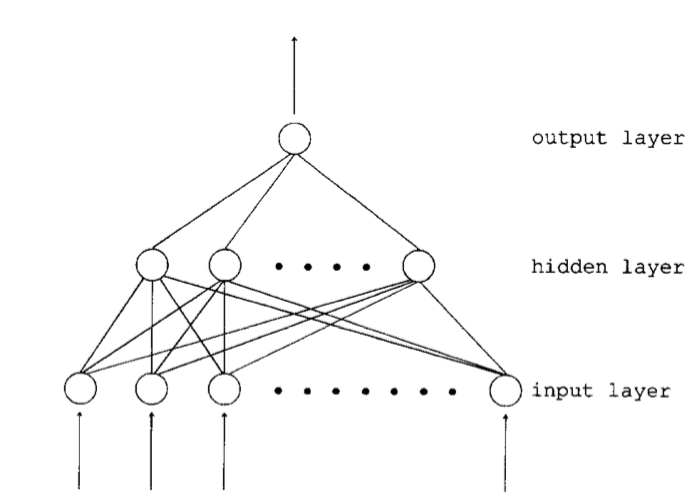
\includegraphics[width=0.6\textwidth]{figures/ff}
            \caption{Typical feed-forward neural network composed of three layers. \cite{svozil1997quantum}}
            \label{fig:ff}
        \end{figure}
    \end{center}
\textbf{Convolutional Neural Networks (CNNs)}\\
These networks are specialized for processing images and are commonly used in computer vision tasks. They use convolutional layers to extract features from images and can learn to recognize patterns and objects in images see in fig~\ref{fig:cn}
    \begin{center}
        \begin{figure}[!ht]
            \centering
            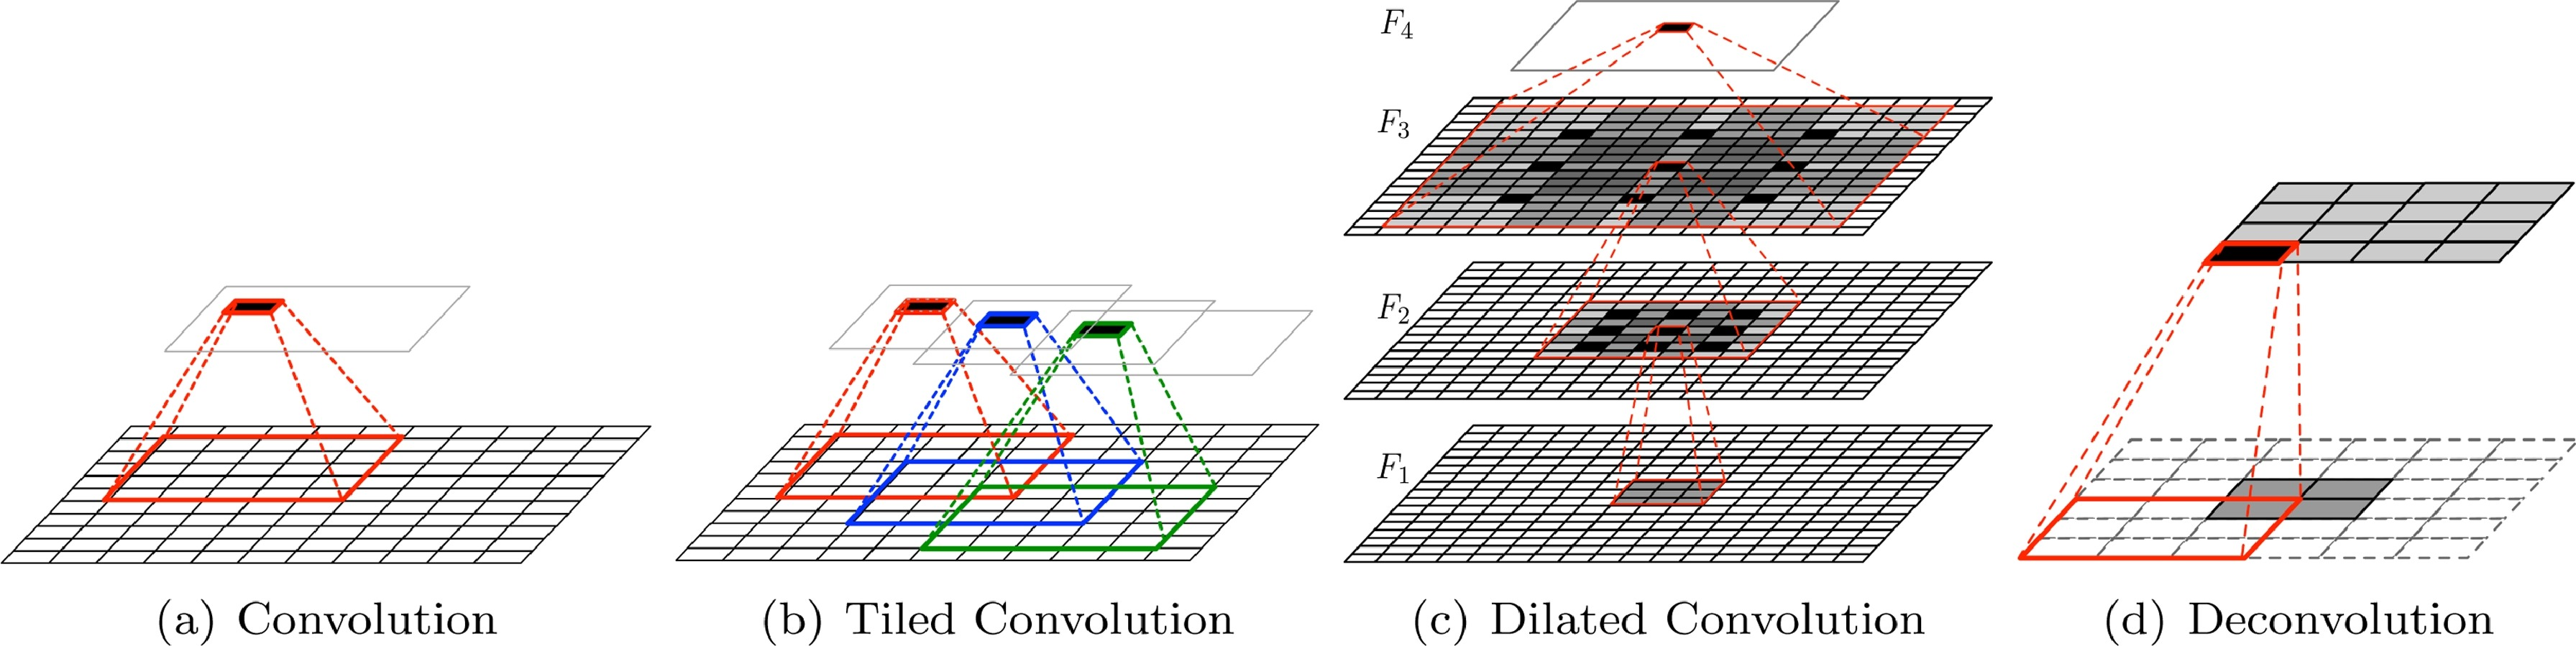
\includegraphics[width=0.8\textwidth]{figures/cn}
            \caption{Illustration of (a) Convolution, (b) Tiled Convolution, (c) Dilated Convolution, and (d)
                Deconvolution. \cite{GU2018354}}
            \label{fig:cn}
        \end{figure}
    \end{center}
\textbf{Recurrent Neural Networks (RNNs)}\\
These networks are designed to work with sequential data, such as time-series or natural language data. They have loops that allow information to be passed from one time-step to~the~next, enabling them to capture temporal dependencies in~the~data, described on fig~\ref{fig:rn}
    \begin{center}
        \begin{figure}[!ht]
            \centering
            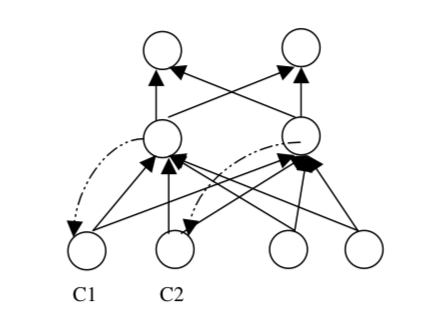
\includegraphics[width=0.8\textwidth]{figures/rn}
            \caption{Typical recurrent network. \cite{medsker2001recurrent}}
            \label{fig:rn}
        \end{figure}
    \end{center}
\textbf{Long Short-Term Memory Networks (LSTMs)}\\
These are~a~type of RNN that are designed to address~the~problem of vanishing gradients in traditional RNNs. They use memory cells and gates to selectively retain or forget information over time, making them well-suited for learning from long sequences. As you can see on fig~\ref{fig:ltmn} color indicates degree of memory activation.
    \begin{center}
        \begin{figure}[!ht]
            \centering
            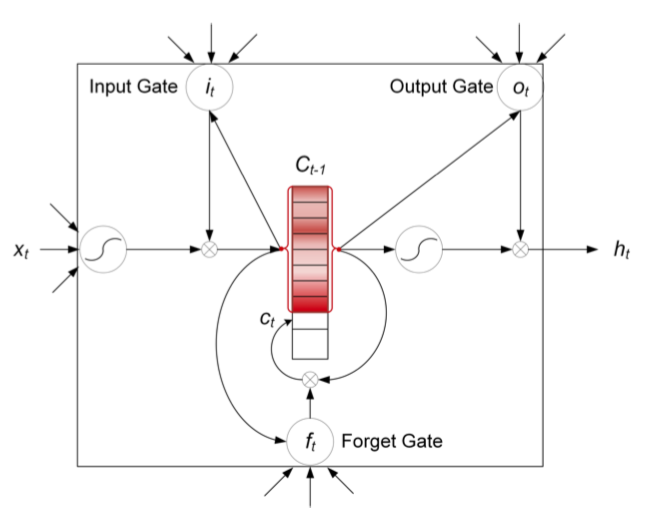
\includegraphics[width=0.4\textwidth]{figures/ltmn}
            \caption{Long short-term memory network. \cite{cheng2016long}}
            \label{fig:ltmn}
        \end{figure}
    \end{center}
\textbf{Autoencoder Neural Networks}\\
These networks are used for unsupervised learning and are designed to learn~a~compressed representation of~the~input data. As we can see on figure~\ref{fig:ann} they consist of~an~encoder that maps~the~input data to~a~compressed representation, and~a~decoder that maps~the~compressed representation back to~the~original data.
    \begin{center}
        \begin{figure}[!ht]
            \centering
            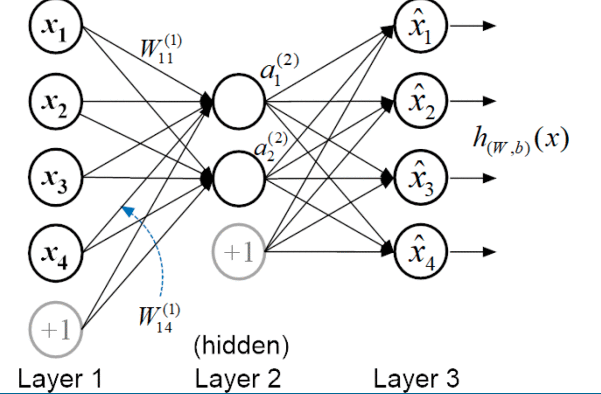
\includegraphics[width=0.5\textwidth]{figures/ann}
            \caption{An autoencoder neural network. \cite{luo2018distributed}}
            \label{fig:ann}
        \end{figure}
    \end{center}
\textbf{Generative Adversarial Networks (GANs)}\\
These networks consist of two networks,~a~generator and~a~discriminator (see on figure~\ref{fig:gan}), that are trained together in~a~game-theoretic framework.~the~generator is trained to generate realistic data samples, while~the~discriminator is trained to distinguish between real and generated data samples.
    \begin{center}
        \begin{figure}[!ht]
            \centering
            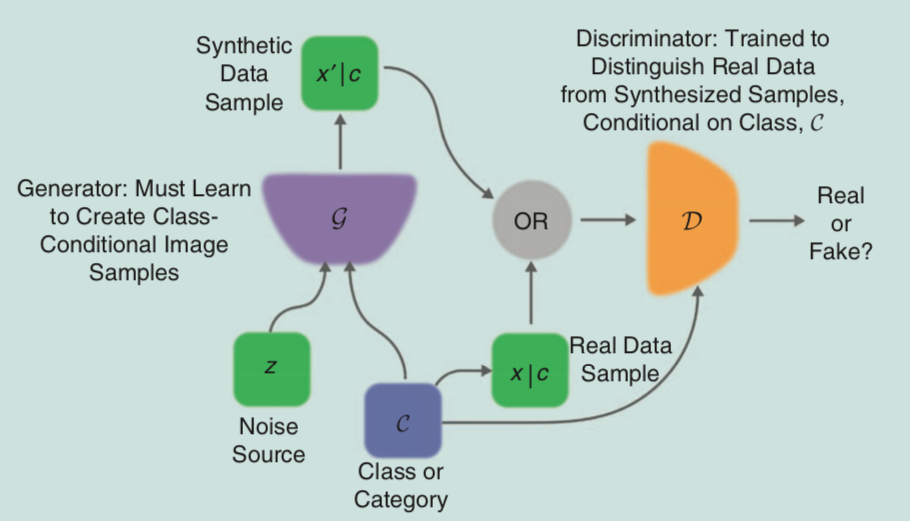
\includegraphics[width=0.5\textwidth]{figures/gan}
            \caption{The conditional GAN schema. \cite{creswell2018generative}}
            \label{fig:gan}
        \end{figure}
    \end{center}

These are some of~the~most common types of neural networks, but there are many other specialized types of neural
networks that have been developed for specific tasks, such as object detection, speech recognition, and
natural language processing.\\

\subsection{Classification} \label{subsec:clasification}
Neural network data classification is~a~technique for categorizing data into different classes or categories based on
patterns and features present in~the~data.~a~neural network is~a~type of machine learning algorithm that is modeled
after~the~structure and function of~the~human brain. It is composed of interconnected nodes or neurons that are
organized into layers.\\
In~a~classification task,~the~neural network is trained on~a~dataset that is labeled with~the~correct
class for each example. During training,~the~network learns to recognize patterns and features in~the~input data
that are associated with each class.~the~process of training involves adjusting~the~weights and biases of~the~neurons
in~the~network to minimize~the~error between~the~predicted class and~the~actual class of each example in the
training set.\\
Once~the~neural network is trained, it can be used to classify new, unseen examples by inputting~the~data into
the network and obtaining~a~prediction of~the~most likely class.~the~output of~the~neural network is~a~probability
distribution over~the~different classes, with~the~highest probability indicating~the~predicted class.\\
Neural network data classification has been successfully applied to~a~wide range of tasks, including image
classification, speech recognition, natural language processing, and fraud detection, among others~\cite{feraud2002methodology}.

\subsection{Activation functions} \label{subsec:nnaf}
There are several types of activation functions~\cite{geron2022hands} used in neural networks, as we can see on figure~\ref{fig:activationfunctions} including:
\begin{itemize}
    \item Sigmoid Function:~the~sigmoid function is~a~commonly used activation function that maps any input value
    to~a~value between 0 and 1. It is typically used in binary classification problems and in~the~output layer of
    neural networks that produce probability estimates~\ref{fig:sigmoid}.
    \item ReLU (Rectified Linear Unit):~the~ReLU function is another popular activation function that maps any
    input value less than 0 to 0, and any input value greater than or equal to 0 to~the~input value itself.
    It is computationally efficient and has been shown to work well in deep neural networks~\ref{fig:relu}.
    \item Tanh Function:~the~tanh (hyperbolic tangent) function is similar to~the~sigmoid function,
    but it maps input values to~a~range between -1 and 1. It is commonly used in~the~hidden layers of neural networks~\ref{fig:tahn}.
    \item Softmax Function:~the~softmax function is often used in~the~output layer of neural networks that produce
    multi-class classification predictions. It maps~the~outputs to~a~probability distribution over~the~possible classes~\ref{fig:sigmsoftmaxoid}.
    \item Leaky ReLU:~the~Leaky ReLU function is similar to~the~ReLU function, but it allows~a~small, non-zero
    gradient when~the~input value is negative. This can help to prevent~the~"dying ReLU" problem, where some ReLU
    units become inactive and stop contributing to~the~network's output~\ref{fig:leakyrelu}.
    \item ELU (Exponential Linear Unit):~the~ELU function is similar to~the~ReLU function, but it allows negative
    values to have non-zero outputs. This can help to prevent~the~"dying ReLU" problem and can improve the
    performance of deep neural networks~\ref{fig:elu}.
\end{itemize}
These are some of~the~most commonly used activation functions in neural networks, but there are many other types of
activation functions that have been developed for specific tasks or to address certain problems.

\begin{figure}
    \centering
    \begin{subfigure}[b]{0.4\textwidth}
        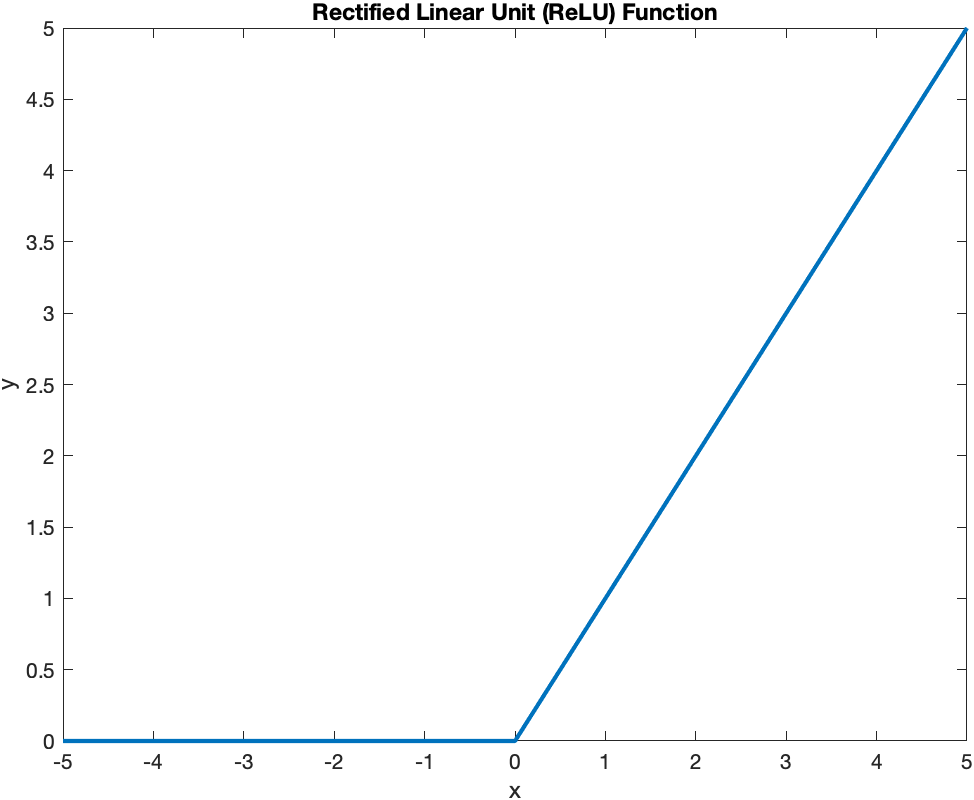
\includegraphics[width=\textwidth]{figures/relu}
        \caption{ReLU function}
        \label{fig:relu}
    \end{subfigure}
    \hspace{0.1\textwidth}
    \begin{subfigure}[b]{0.4\textwidth}
        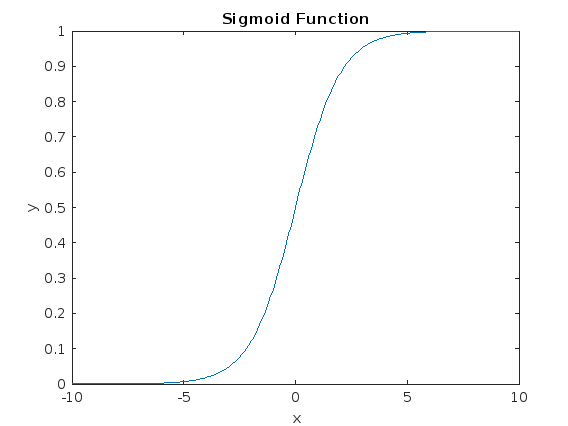
\includegraphics[width=\textwidth]{figures/sigmoid}
        \caption{Sigmoid function}
        \label{fig:sigmoid}
    \end{subfigure}
    \begin{subfigure}[b]{0.4\textwidth}
        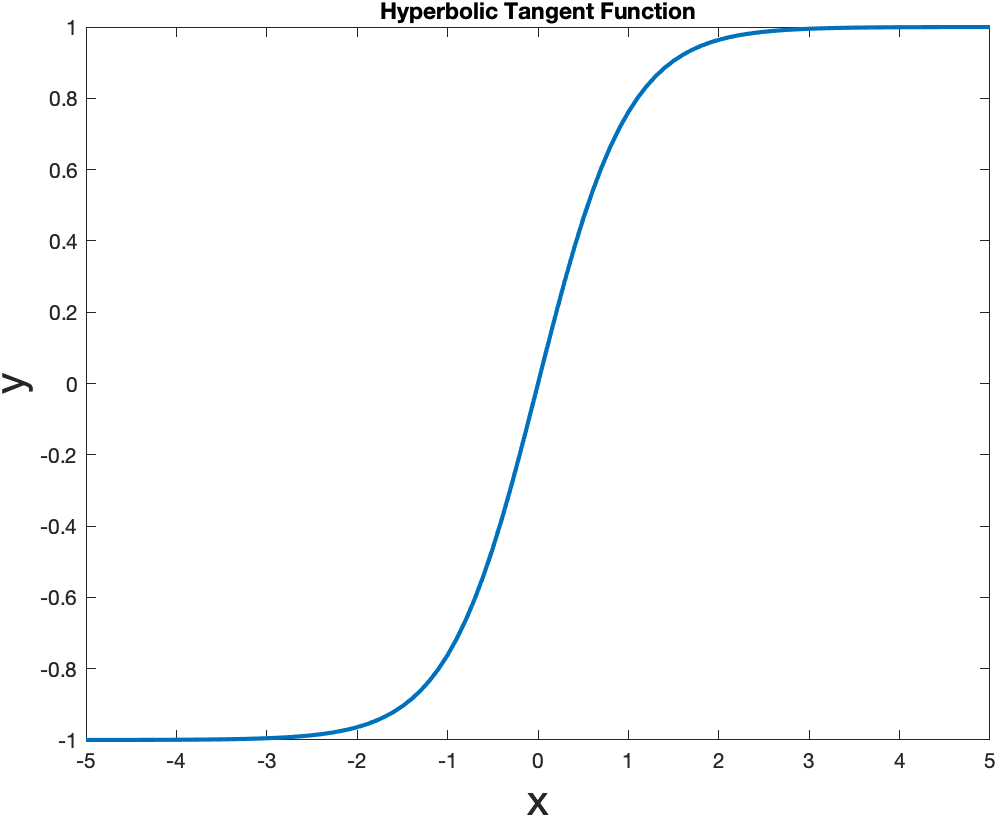
\includegraphics[width=\textwidth]{figures/tanh}
        \caption{Tanh function}
        \label{fig:tahn}
    \end{subfigure}
    \hspace{0.1\textwidth}
    \begin{subfigure}[b]{0.4\textwidth}
        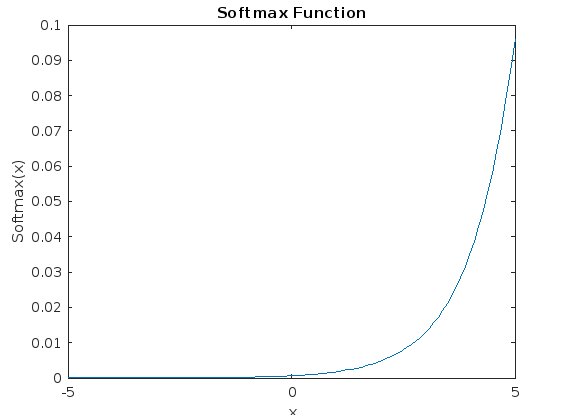
\includegraphics[width=\textwidth]{figures/softmax}
        \caption{Softmax function}
        \label{fig:sigmsoftmaxoid}
    \end{subfigure}
    \begin{subfigure}[b]{0.4\textwidth}
        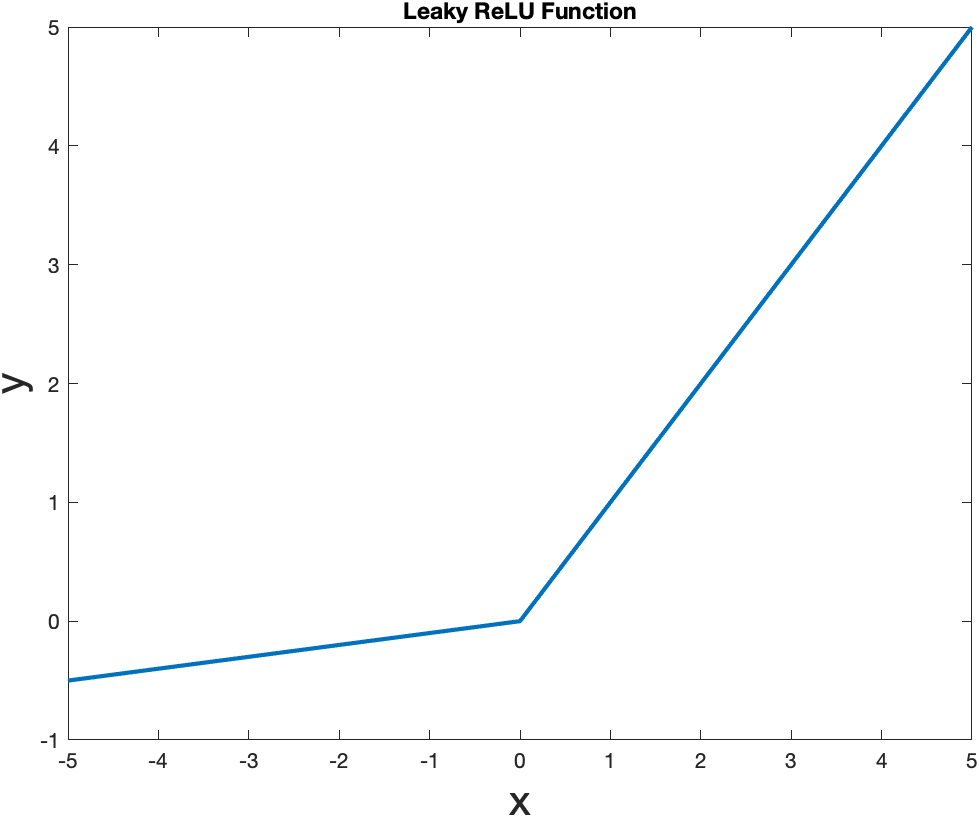
\includegraphics[width=\textwidth]{figures/leakyrelu}
        \caption{Leaky ReLU function}
        \label{fig:leakyrelu}
    \end{subfigure}
    \hspace{0.1\textwidth}
    \begin{subfigure}[b]{0.4\textwidth}
        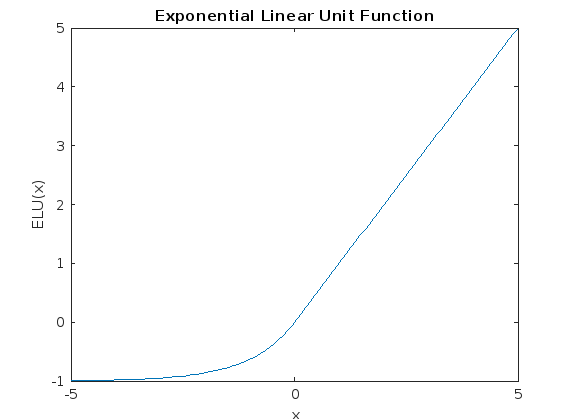
\includegraphics[width=\textwidth]{figures/elu}
        \caption{ELU function}
        \label{fig:elu}
    \end{subfigure}
    \caption{Neural network activation functions.}
    \label{fig:activationfunctions}
\end{figure}

\subsection{Application of neural netwrok in prediction} \label{subsec:nnprediction}
Neural networks can be used for long-term linear prediction in time-series data, including speech, health, and
stock data. Neural networks can be trained to model and forecast~the~patterns in~the~data, including shifts in
the long-term linear prediction. Neural networks have been shown to be effective in capturing~the~complex relationships
between variables in time-series data, and can learn to identify subtle patterns and trends that may be difficult
to detect using traditional statistical methods. In~the~context of long-term linear prediction, neural networks can be
trained on historical data to identify prev    atterns and trends in~the~data and make predictions for future values.
They can also be used to detect shifts in~the~long-term linear prediction, which can be useful for identifying
changes in~the~underlying processes that generate~the~data. However, it's important to note that neural networks
can be computationally expensive and require large amounts of data to train effectively. They also require careful
tuning of hyperparameters and selection of appropriate architecture to achieve good performance.
In addition,~the~interpretation of~the~results of~a~neural network can be more challenging than with traditional
statistical methods. Overall, neural networks can be~a~powerful tool for long-term linear prediction in time-series
data, including shifts in~the~data, but their use should be carefully considered based on~the~specific
application and available data.


\section{Linear prediction} \label{sec:lp}
Linear prediction is~a~statistical technique used to forecast future values based on past observations. It is~a~method
for modeling~the~relationship between~a~dependent variable and one or more independent variables in~a~linear form.
The goal of linear prediction is to find~the~best linear approximation of~the~relationship between~the~variables,
which can then be used to make predictions about future values of~the~dependent variable.
\\
Linear prediction can be performed using simple linear regression or multiple linear regression, depending on the
number of independent variables involved~\cite{Parks}. In simple linear regression,~a~single independent variable is
used to predict~the~value of~the~dependent variable, while in multiple linear regression, multiple independent
variables are used to make~the~prediction.
\\
Linear prediction models are commonly used in finance, economics, and engineering, among other fields, to forecast
future values of time series data, such as stock prices, sales, or demand.~the~accuracy of linear prediction models
depends on several factors, including~the~quality of~the~data,~the~choice of independent variables, and~the~degree of
linearity in~the~relationship between~the~variables.

\subsection{Short-term linear prediction} \label{subsec:shortlp}

Short-term linear prediction~\cite{Riahy} refers to~the~use of linear prediction techniques to make predictions about
the near-term future values of~a~time series. It is used to forecast future values of~a~dependent variable based on
its past values and any relevant independent variables.
\\
In short-term linear prediction,~the~focus is on accurately predicting~the~next few values of~the~dependent variable,
typically in~the~range of several weeks to~a~few months.~the~linear prediction models used for short-term
forecasting are typically simple and straightforward, often using~a~small number of independent variables.
The goal is to provide~a~quick and easily interpretable forecast that can be used to make operational decisions in
the short-term.
Consider~a~signal $x(n)$ that is modeled using~a~linear predictor.~the~linear predictor is defined as:

\begin{equation}
  \hat{x}(n) = \sum_{i=1}^{p} a_i x(n-i),
  \label{eq:linear-predictor}
\end{equation}

where $\hat{x}(n)$ is~the~predicted value of $x(n)$, $p$ is~the~order of~the~predictor, and $a_i$ are~the~predictor coefficients.~the~predictor coefficients can be found by minimizing~the~prediction error:

\begin{equation}
  e(n) = x(n) - \hat{x}(n),
  \label{eq:prediction-error}
\end{equation}

Using~the~least squares method, we can find~the~predictor coefficients by minimizing~the~sum of squared prediction errors:

\begin{equation}
  \min_{a_1,\dots,a_p} \sum_{n=1}^{N} e^2(n),
  \label{eq:least-squares}
\end{equation}

This can be solved analytically using~the~following matrix equation:

\begin{equation}
  \begin{bmatrix}
    r(0) & r(1) & \cdots & r(p-1) \\
    r(1) & r(0) & \cdots & r(p-2) \\
    \vdots & \vdots & \ddots & \vdots \\
    r(p-1) & r(p-2) & \cdots & r(0)
  \end{bmatrix}
  \begin{bmatrix}
    a_1 \\
    a_2 \\
    \vdots \\
    a_p
  \end{bmatrix}
  =
  \begin{bmatrix}
    r(1) \\
    r(2) \\
    \vdots \\
    r(p)
  \end{bmatrix},
  \label{eq:matrix-equation}
\end{equation}

where $r(k)$ is~the~autocorrelation function of~the~signal $x(n)$ defined as:

\begin{equation}
  r(k) = \frac{1}{N} \sum_{n=k+1}^{N} x(n) x(n-k),
  \label{eq:autocorrelation}
\end{equation}

Common techniques for short-term linear prediction include moving average models, exponential smoothing, and
autoregressive models. These methods use~the~historical data of~the~time series to model~the~relationship between the
dependent and independent variables, and to make predictions about future values.~the~accuracy of short-term linear
predictions can be evaluated using metrics such as mean absolute error, mean squared error, or~the~correlation
coefficient between~the~actual and predicted values.

\subsection{Long-term linear prediction}\label{subsec:longlp}
Long-term linear prediction is~a~technique commonly used in~the~analysis of time-series data, including health data.
In~the~context of health data,~the~shift of long-term linear prediction refers to~the~way in which~the~patterns in the
data change over time, reflecting changes in~the~underlying health status of~the~individual or population being studied.\\
For example, in~the~case of~a~patient with~a~chronic disease,~the~long-term linear prediction of their health data may
show~a~gradual decline over time as~the~disease progresses. Alternatively,~the~data may show periodic shifts
corresponding to changes in medication or other interventions. In population health studies, long-term linear
prediction can be used to identify trends and patterns in health outcomes over time. For example,~a~long-term linear
prediction model might be used to track changes in~the~prevalence of~a~particular disease or condition
over~a~period of several years, taking into account factors such as demographic changes and changes in healthcare policy.
Overall,~the~shift of long-term linear prediction for health data reflects~the~dynamic nature of health status and
healthcare interventions, and can be~a~powerful tool for understanding trends and patterns in health outcomes over time.
\\
Long-term linear prediction refers to~the~use of linear prediction techniques to make predictions about~the~future
values of~a~time series over~an~extended period of time, typically several months to several years. Unlike short-term
linear prediction, which focuses on forecasting~the~near-term future, long-term linear prediction aims to provide~a~more
comprehensive and accurate forecast of future values.\\
\begin{equation}/label(eq:ltlp)
    \hat{x}(n) = \sum_{i=1}^{p} a_i x(n-i) + \sum_{i=1}^{q} b_i e(n-T-i),
\end{equation}
\\
where $\hat{x}(n)$ is~the~predicted value of~the~signal at time $n$, $x(n-i)$ are~the~past $p$ samples of~the~signal, $e(n-i)$ are~the~past $q$ prediction errors, and $a_i$ and $b_i$ are~the~predictor coefficients.~the~order of~the~predictor is $p$ for~the~autoregressive (AR) part and $q$ for~the~moving average (MA) part.

The long-term linear prediction equation is~a~generalization of~the~short-term linear prediction equation that was shown in section~\ref{subsec:shortlp}.~the~short-term equation only includes~the~autoregressive (AR) part, whereas~the~long-term equation includes both~the~autoregressive (AR) and~the~moving average (MA) parts.

In long-term linear prediction, more sophisticated models~\cite{Nave} are typically used, such as multiple linear
regression or time series models, and~a~larger number of independent variables may be considered.~the~models are also
trained on~a~larger historical dataset to ensure that they capture any long-term trends or patterns in~the~data.
\\
Long-term linear prediction is commonly used in fields such as finance, economics, and marketing, to make long-term
projections about variables such as sales, demand, or stock prices.~the~goal is to provide~a~comprehensive and accurate
forecast that can be used to make strategic decisions in~the~long-term.~the~accuracy of long-term linear predictions
can be evaluated using~the~same metrics as for short-term linear predictions~\cite{Baker}, as well as additional metrics
such as mean absolute percentage error or mean absolute scaled error.
\\
In some long-term prediction use cases it needs to solve~the~suppression of Late Reverberation
Effect\footnote{Late Reverberation Effect refers to~the~decay of sound in~an~environment after~the~initial sound source
has stopped. This effect results in~the~persistence of sound in~a~space for~a~short period of time and helps create the
characteristic ambiance of~a~room or space. It is~an~important aspect of room acoustics and is used in sound
design and music production to enhance~the~perceived sound quality and spatial experience of audio.} this can be done
by with minimal performance degradation by framework developed by Keisuke Kinoshita~\cite{Kinoshita} for both
single-channel and multichannel scenarios.\\
\\
\textbf{Shift Estimation}\\

The shift of long-term linear prediction for example in human speech refers to~the~way in which~the~human vocal system produces sounds over time.
Specifically, it describes~the~changes that occur in~the~speech signal over relatively long periods of time, typically
measured in tens to hundreds of milliseconds. Long-term linear prediction is~a~technique used in speech analysis and
synthesis to model~the~way that~the~vocal system produces speech sounds. It involves breaking~the~speech signal into
short segments and using mathematical algorithms to predict~the~signal in each segment based on~the~signal in preceding
segments.~the~shift of long-term linear prediction in human speech refers to~the~fact that~the~vocal system is constantly
adjusting and adapting~the~way that it produces sounds based on~a~variety of factors, including~the~phonemes being spoken,
the speaker's emotions and intentions, and~the~context of~the~speech. This means that~the~speech signal is not static,
but rather is constantly shifting and evolving over time. For example, when~a~speaker is emphasizing~a~particular
word or phrase, they may change~the~pitch, intensity, or duration of certain sounds in order to convey their meaning
more effectively. These changes will be reflected in~the~long-term linear prediction of~the~speech signal, which will
show shifts in~the~predicted signal over time.\\
\\
In~the~context of stock data analysis,~the~shift in long-term prediction refers to~the~way in which~the~patterns in
the data change over time, reflecting changes in~the~underlying market conditions and investor sentiment.
Long-term linear prediction is~a~technique that can be used to model and forecast stock prices based on historical
price data. It involves breaking~the~time-series data into short segments and using mathematical algorithms to predict
the price in each segment based on~the~price in preceding segments.~the~shift in long-term prediction for stock data
can occur due to~a~variety of factors such as changes in~the~macroeconomic environment, company earnings announcements,
news events, investor sentiment, and other market-moving events. These shifts can cause changes in~the~underlying trends
and patterns in~the~data, which can make it difficult to accurately predict stock prices over longer time horizons.
For example, sudden changes in market conditions such as~a~global financial crisis or~a~political event can cause
significant shifts in long-term prediction for stock data, making it difficult to accurately forecast future prices.
Similarly,~a~company's financial performance or regulatory changes can cause sudden shifts in~the~long-term prediction
for that company's stock. Overall,~the~shift in long-term prediction for stock data reflects~the~dynamic and
unpredictable nature of~the~stock market, and underscores~the~importance of using multiple sources of data and analysis
techniques to make informed investment decisions.\\
\\
To calculate~the~shift for long-term linear prediction, we can use~the~autocorrelation function of~the~signal.
The shift value corresponds to~the~lag at which~the~autocorrelation function has its maximum value. Other approaches to estimate shift we can see in section~\ref{sec:patterns}


\subsection{Estimation of Optimal Predictor Order} \label{subsec:orderlp}
The optimal order of linear prediction refers to~the~number of past observations that should be used to predict~the~next
observation in~a~time series. There are several methods for finding~the~optimal order of linear prediction, including
the Akaike Information Criterion (AIC),~the~Bayesian Information Criterion (BIC), and cross-validation.~the~Akaike
Information Criterion (AIC) is~a~measure of~the~relative quality of~a~statistical model for~a~given set of data.
The AIC score is based on~the~goodness of fit of~the~model and~the~complexity of~the~model. In~the~context of linear
prediction,~the~AIC can be used to select~the~optimal order of~the~autoregressive (AR) model.~the~AR model uses past
observations to predict~the~next observation in~a~time series.~the~optimal order of~the~AR model is~the~order that
minimizes~the~AIC score.~the~Bayesian Information Criterion (BIC) is similar to~the~AIC but places~a~greater penalty
on model complexity.~the~BIC can also be used to select~the~optimal order of~the~AR model. Cross-validation is a
technique that involves splitting~the~data into training and testing sets.~the~model is trained on~the~training set, and
the performance of~the~model is evaluated on~the~testing set.~the~optimal order of~the~AR model is~the~order that produces
the best performance on~the~testing set. Overall,~the~optimal order of linear prediction can be found using~a~combination
of these methods, taking into account~the~complexity of~the~model,~the~goodness of fit, and~the~performance on~a~testing set.\\
\\
Autocorrelation can be~a~useful tool for detecting~the~optimal shift in long-term linear prediction for time-series data.
Autocorrelation measures~the~linear relationship between lagged versions of~a~time-series, and can be used to identify
the presence of cyclic patterns in~the~data. In~the~context of long-term linear prediction, autocorrelation can be
used to identify~the~lag that maximizes~the~correlation between past and future values of~the~time-series. This lag can
be used as~the~optimal shift for~the~long-term linear prediction model. To use autocorrelation for detecting~the~optimal
shift in long-term prediction, one would first calculate~the~autocorrelation function (ACF) for~the~time-series data.
The ACF measures~the~correlation between~the~time-series at different lags.~the~lag at which~the~ACF is highest
corresponds to~the~optimal shift for long-term linear prediction. Once~the~optimal shift has been identified, it can
be used to train~a~long-term linear prediction model using techniques such as autoregressive models, moving average
models, or combinations of both. However, it's important to note that while autocorrelation can be~a~useful tool for
identifying~the~optimal shift for long-term linear prediction, it may not always be~the~most appropriate technique for
all types of time-series data. Other methods, such as spectral analysis or wavelet analysis, may be more
appropriate in some cases.\\
\\
Autocorrelation function (ACF) of~a~time series is typically denoted as $\rho_k$ or $r_k$ and can be expressed
mathematically using~the~following equation:
\begin{equation}
    \rho_k = \frac{\gamma_k}{\gamma_0} = \frac{\sum_{t=k+1}^{T}(y_t - \bar{y})(y_{t-k} - \bar{y})}{\sum_{t=1}^{T}(y_t - \bar{y})^2},
\end{equation}
where $y_t$ is~the~value of~the~time series at time $t$, $\bar{y}$ is~the~mean of~the~time series, $k$ is~the~lag or
time shift, $\gamma_k$ is~the~autocovariance at lag $k$, $\gamma_0$ is~the~autocovariance at lag 0, and $T$ is~the~total number
of observations in~the~time series.~the~ACF measures~the~correlation between~the~time series and~a~lagged version of
itself, with values ranging between -1 and 1.

\subsection{Levinson-Durbin scheme} \label{subsec:levinson}

The Levinson-Durbin algorithm~\cite{Levinson} is~an~iterative numerical method used to solve~the~autoregressive
(AR) model of~a~time series.

\begin{equation}
    \label{eq:levinson}
    Y_t = \beta_0 + \beta_1 Y_{t-1} + \beta_2 Y_{t-2} + \cdots + \beta_p Y_{t-p} + \epsilon_t,
\end{equation}

where $Y_t$ is~the~dependent variable at time $t$, $\beta_0$ is~the~intercept, $\beta_1, \beta_2, \dots, \beta_p$ are the
regression coefficients, $Y_{t-1}, Y_{t-2}, \dots, Y_{t-p}$ are~the~lagged values of~the~dependent variable up to
order $p$, and $\epsilon_t$ is~the~error term at time $t$.

AR models are used to model and forecast time series data~\cite{Durbin}, such as sales data, by assuming that each
future value of~the~series depends on~a~linear combination of previous values.
\\
The Levinson-Durbin algorithm solves~the~AR model by iteratively updating~the~coefficients of~the~model to minimize
the prediction error between~the~model and~the~actual data.~the~algorithm is fast and efficient, and it is widely
used in digital signal processing, speech processing, and control systems, among other applications.
The Levinson-Durbin recursion schema is~a~method for solving~the~autocorrelation equations of~a~linear
prediction problem. It can be expressed in~the~form of~a~triangular system of equations:

\begin{equation*}
    \begin{aligned}
        \alpha_0 &= r_0 \\
        \alpha_k &= \frac{1}{k} \sum_{i=1}^{k} a_{k-i} r_i \quad (1 \leq k < p) \\
        \alpha_p &= \frac{1}{p} \sum_{i=1}^{p} a_{p-i} r_i,
    \end{aligned}
\end{equation*}
\\
where $r_i$ is~the~$i$th autocorrelation coefficient, $\alpha_k$ is~the~$k$th reflection coefficient, and $a_k$ is~the~$k$th
prediction coefficient.
\\
The recursion begins with $\alpha_0 = r_0$, and computes each subsequent reflection coefficient $\alpha_k$ in terms of the
previous coefficients $\alpha_0, \alpha_1, \ldots, \alpha_{k-1}$ and~the~autocorrelation coefficients $r_1, r_2, \ldots, r_k$.\\
The Levinson-Durbin algorithm is often used as~an~alternative to~the~Yule-Walker equations, which are another commonly
used method for solving AR models. Unlike~the~Yule-Walker equations,~the~Levinson-Durbin algorithm can be easily
modified to handle non-stationary time series data, and it is also more robust to numerical issues such as
rounding errors.\\
\begin{equation*}
    \begin{bmatrix}
        r_0     & r_1     & \cdots & r_{p-1} \\
        r_1     & r_0     & \cdots & r_{p-2} \\
        \vdots  & \vdots  & \ddots & \vdots  \\
        r_{p-1} & r_{p-2} & \cdots & r_0
    \end{bmatrix}
    \begin{bmatrix}
        a_1    \\
        a_2    \\
        \vdots \\
        a_p
    \end{bmatrix}
    =
    \begin{bmatrix}
        -r_1   \\
        -r_2   \\
        \vdots \\
        -r_p
    \end{bmatrix},
\end{equation*}

where $r_0, r_1, \ldots, r_{p-1}$ are~the~autocorrelation coefficients and $a_1, a_2, \ldots, a_p$ are~the~prediction coefficients.~the~algorithm proceeds as follows:\\

\begin{enumerate}
    \item Set $\alpha_0 = r_0$ and $k = 1$.
    \item Compute~the~reflection coefficient $\alpha_k$ using~the~formula

    \begin{equation*}
        \alpha_k = -\frac{1}{\alpha_{k-1}} \sum_{i=1}^{k-1} \alpha_{k-i} r_i.
    \end{equation*}

    \item Compute~the~new prediction coefficients $a_1, a_2, \ldots, a_k$ using~the~formulas

    \begin{align*}
        a_k &= -\alpha_k \\
        a_i &= a_{i-1} - \alpha_k a_{k-i} \quad (1 \leq i < k).
    \end{align*}

    \item If $k = p$, terminate. Otherwise, increment $k$ and repeat from step 2.
\end{enumerate}


\section{Detection of repeatable patterns}\label{sec:patterns}
To detect repeatable patterns in time series data, we can use several techniques. As a basic method Autocorrelation is used to measures~the~correlation between~the~time series data at different time lags~\ref{subsec:orderlp}. The next one which is mainly use is th Seasonal decomposition~\ref{subsec:seasonal} which separates~the~time series data into different components
such as trend, seasonal, and residual. To analyze~the~frequency components of~the~time series data Fourier transform~\ref{subsec:fourier} can be used. Same as another mathematical technique to analyze~the~time-frequency structure of~the~time series data called Wavelet analysis.
To detect pattern in seasonal trends Hidden Markov models~\ref{subsec:hmm} can be used.
These models assume that~the~data follows~a~probabilistic process, where~the~state of~the~process is not directly observable. The last one method which is as much as used is the Pattern Masking for Dictionary Matching (PMDM)~\ref{subsec:pmdm}.\\
These techniques can be used individually or in combination to detect repeatable patterns in time series data. It's important to note that~the~choice of technique depends on~the~characteristics of~the~data and~the~specific problem being addressed.


\subsection{Hidden Markov models}\label{subsec:hmm}
Hidden Markov Models (HMMs) are probabilistic models that are used to analyze sequential data where~the~state of the
system is not directly observable. HMMs consist of~a~set of hidden states that are not directly observable, and a
set of observable symbols that are emitted from~the~hidden states~\cite{math10081230}.\\
\\
The HMM assumes that~the~hidden states form~a~Markov chain, which means that~the~probability of transitioning from
one hidden state to another depends only on~the~current state and not on~the~previous states.~the~emission
probabilities of~the~observable symbols depend only on~the~current hidden state.\\
\\
HMMs are typically used for two main tasks:
\begin{itemize}
    \item Evaluation: Given~a~sequence of observable symbols, HMMs can be used to evaluate~the~probability of the
    sequence of symbols occurring, given~a~particular set of model parameters.
    \item Decoding: Given~a~sequence of observable symbols, HMMs can be used to determine~the~most likely
    sequence of hidden states that generated~the~sequence of symbols.
    \item HMMs are used in~a~wide range of applications such as speech recognition, handwriting recognition, natural
    language processing, bioinformatics, and financial time series analysis.
\end{itemize}
The basic steps involved in building~an~HMM model are as follows:
\begin{enumerate}
    \item Define~the~set of hidden states: Determine~the~set of hidden states that~the~system can be in at any given time.
    \item Define~the~set of observable symbols: Determine~the~set of observable symbols that can be emitted from each hidden state.
    \item Define~the~transition probabilities: Determine~the~probability of transitioning from one hidden state to another.
    \item Define~the~emission probabilities: Determine~the~probability of emitting each observable symbol from each hidden state.
    \item Estimate~the~model parameters: Estimate~the~transition and emission probabilities of~the~HMM using~a~training dataset.
    \item Use~the~model for evaluation or decoding: Once~the~model parameters have been estimated,~the~HMM
    can be used for evaluation or decoding tasks.
\end{enumerate}
It's important to note that building~an~HMM model requires knowledge of probability theory and statistical
modeling, and may require significant computational resources.



\subsection{Fourier transform}\label{subsec:fourier}
Fourier transform is~a~mathematical technique that is used to analyze~the~frequency components of~a~signal or~a~time
series data. It transforms~a~signal from~the~time domain into~the~frequency domain, which allows us to analyze the
signal in terms of its frequency components.~the~Fourier transform is widely used in many fields, including signal
processing, image processing, and physics.\\
\\
The Fourier transform decomposes~a~signal into~a~set of sinusoidal waves with different frequencies, amplitudes, and phases.
These sinusoidal waves are called~the~Fourier series, and they represent~the~signal as~a~sum of complex exponential functions.\\
\\
The Fourier transform can be expressed as~an~integral equation that takes~a~time-domain signal and
produces~a~frequency-domain representation of that signal.~the~formula for~the~Fourier transform is:\\
\begin{equation}
    F(\omega) = \int f(t) e^{(-i \omega t)} dt,
\end{equation}
where $F(\omega)$ is~the~frequency-domain representation of~the~signal, $f(t)$ is~the~time-domain signal, $\omega$ is the
frequency, and i is~the~imaginary unit.\\
\\
The inverse Fourier transform can be used to transform~the~frequency-domain representation of~a~signal back into the
time domain.~the~formula for~the~inverse Fourier transform is:
\begin{equation}
    f(t) = \frac{1}{2\pi} \int F(\omega) e^{(i \omega t)} d\omega,
\end{equation}
where $f(t)$ is~the~time-domain signal, $F(\omega)$ is~the~frequency-domain representation of~the~signal, $\omega$ is the
frequency, and i is~the~imaginary unit.\\
\\
The Fourier transform has many practical applications. For example, it can be used to analyze~the~frequency components
of~a~music signal, to filter out noise from~a~signal, or to compress data by removing high-frequency components that
are not essential for~the~representation of~the~signal.  It is~a~powerful tool for understanding~the~underlying
structure of signals and is widely used in scientific research and engineering applications.

\subsection{Seasonal decomposition}\label{subsec:seasonal}
Seasonal decomposition is~a~statistical technique that is used to decompose~a~time series into its underlying components,
including trend, seasonal, and residual components. This technique is useful for identifying and understanding
the repeating patterns or seasonal effects in~a~time series data.\\
\\
The seasonal decomposition of~a~time series involves separating~the~data into four components:
\begin{itemize}
    \item Trend component represents~the~long-term pattern in~the~data, such as increasing or
    decreasing trends over time.
    \item Seasonal component represents~the~repeating pattern in~the~data that occurs over~a~fixed
    period, such as daily, weekly, or monthly patterns.
    \item Residual component represents~the~remaining variation in~the~data that cannot be explained
    $y$~the~trend or seasonal components. It may include random noise or other unexplained factors.
    \item Irregular component represents any unexpected or irregular variation in~the~data that is not
    accounted for by~the~other components.
\end{itemize}
The seasonal decomposition process involves applying~a~smoothing algorithm to~the~time series data to estimate the
trend and seasonal components, and then subtracting them from~the~original data to obtain~the~residual component.
There are various methods for performing seasonal decomposition, including moving averages, exponential smoothing,
and regression models.\\
\\
Once~the~components of~the~time series have been separated, they can be analyzed and modeled separately.
This can help in detecting~the~repeating patterns or seasonal effects in~the~data and in making accurate forecasts for
future time periods.\\
\\
Overall, seasonal decomposition is~a~powerful tool for identifying and analyzing~the~seasonal patterns in~a~time series
data, and it can be useful in~a~wide range of applications, including finance, economics, and meteorology.\\

\subsection{Pattern Masking for Dictionary Matching}\label{subsec:pmdm}
Pattern masking is~a~technique used in dictionary matching to find occurrences of words or phrases in~a~given text.
In this technique,~a~pattern  is defined as~a~string of characters that represents~the~word or phrase being searched for.
However, in some cases,~the~exact spelling of~the~word or phrase may not be known, or there may be variations in the
spelling that need to be accounted for.\\
\\
To handle such scenarios, pattern masking is used. In pattern masking, certain characters in~the~pattern are replaced
with special characters that can match~a~range of different characters. For example,~the~asterisk (\*) character can be
used to represent any number of characters, while~the~question mark (?) can represent~a~single character.\\
\\
Here's~an~example to illustrate how pattern masking works. Let's say we want to find occurrences of~the~word
"colour" in~a~given text, but we want to account for variations in spelling such as "color" or "colours".
We can define~a~pattern for this as "colours", where~the~question mark represents~a~single character that
may or may not be present.\\
\\
By using pattern masking, we can search for occurrences of~the~pattern "colou?rs" in~the~text, and it will match
any of~the~variations of~the~word "colour" that we specified in~the~pattern.\\
Dictionary matching algorithms can use pattern masking to search for multiple words or phrases simultaneously,
which can be useful for tasks such as text classification, information retrieval, or sentiment analysis~\cite{pmdm}.

% !TEX root = ../thesis.tex
\chapter{Goal of~the~thesis}\label{sec:goal}
In this thesis we are focus on improving linear prediction in sales and financial forecasting and combine it with
modern machine learning approaches. Machine learning techniques are used to improve~the~accurate of linear
prediction models. Specifically, there are two ways in which machine learning are applied to linear prediction:
\begin{enumerate}
    \item Feature engineering: In this approach, machine learning is used to extract relevant features from~the~input
    signal that can be used as input to~a~linear prediction model.The extracted features can capture complex patterns
    in~the~data that are not captured by~the~raw input. Feature engineering can be done using techniques such as
    principal component analysis, wavelet transform, and Fourier transform.
    \item Model selection and training: In this approach, machine learning is used to select~the~best linear
    model for~the~prediction task and to estimate its parameters from~the~data. This can involve selecting~the~best
    set of input variables for~the~linear model, choosing~the~best regularization parameter to avoid overfitting, and
    optimizing~the~model hyperparameters. Common machine learning algorithms used for linear prediction include linear
    regression, support vector regression, and artificial neural networks.
\end{enumerate}
The goal of long-term linear prediction is to estimate future values of~a~signal or time series based on its past
values using~a~linear model.
The linear prediction model uses~a~set of coefficients to weight past values of~the~signal and produce~a~prediction for
future values.~the~accurate of~the~prediction depends on~the~quality of~the~model and~the~complexity of the
underlying signal. Combine this principles get to us~the~best results from linear prediction over
sales and financial datasets.
\chapter{Methodology}\label{sec:methodology}
    \section{Characteristics of~the~research object}\label{subsec:research_object}
    Sales data and financial datasets are two broad categories of data that have different characteristics and are used
    for different purposes. Here are some general characteristics of each type of dataset:\\
    \\
    \textbf{Sales data}\\
    Typically contains transactional information, such as~the~date, time, location, and amount of~a~purchase. Can include additional information about~the~customer, such as their demographic profile, purchase history, and
    preferences. Often analyzed to understand customer behavior, such as buying patterns, trends, and preferences
    May have seasonal or cyclical patterns, depending on~the~nature of~the~product or service being sold
    Can be used to optimize marketing and sales strategies, such as targeting specific customer segments, promoting
    certain products, or adjusting prices and discounts.\\
    \\
    \textbf{Financial datasets}\\
    Typically contains financial information, such as~the~revenue, expenses, assets, liabilities, and cash
    flow of~a~company or organization can include additional information about~the~market, such as interest rates,
    exchange rates, and stock prices. Often analyzed to evaluate~the~financial performance and health of~a~company,
    such as profitability, solvency, and liquidity. May have regulatory or compliance requirements, such as financial
    reporting standards or tax laws. Can be used to make strategic decisions, such as investment, merger and
    acquisition, or divestiture. Both sales data and financial datasets can be used for forecasting and modeling,
    but they have different analytical techniques and tools. Sales data often requires customer segmentation,
    predictive analytics, and machine learning algorithms, while financial datasets require financial ratio analysis,
    time series forecasting, and risk assessment.
    \section{Methods}\label{subsec:methods}
    In our thesis was used mainly these list of methods like a linear prediction, regression, backpropagation or statistical  measures.
        \subsection{Linear regression}\label{sec:linear}
        Linear regression~\cite{Levinson} attempts to model~the~relationship between two variables by fitting~a~linear
        equation to observed data. One variable is considered to be~an~explanatory variable, and~the~other is
        considered to be~a~dependent variable. For example, we want to relate~the~weights of individuals to their
        heights using~a~linear regression model. Before attempting to fit~a~linear model to observed data, we should
        first determine if there exists~a~relationship between~the~variables of interest. This does not necessarily
        mean that one variable causes~the~other, but that there is some significant association between them.
        To determine~the~strength of relationship~a~scatterplot can be~a~helpful tool.
        If there appears to be no association between~the~proposed explanatory and dependent variables, then
        fitting~a~linear regression model to~the~data probably will not provide~a~useful model.
       ~a~valuable numerical measure of association between two variables is~the~correlation coefficient.
        That is~a~value from $[-1, 1]$ range indicating~the~strength of~the~association of~the~observed data
        for~the~two variables.\\
       ~a~linear regression line has~an~equation of~the~form $Y =~a~+ bX$, where $X$ is~the~explanatory variable
        and $Y$ is~the~dependent variable.~the~slope of~the~line is $b$, and $a$ is~the~intercept.
        Example of some basic linear models:\\
        \begin{equation} \label{eq:4}
        \begin{array}{l@{}l}
            Y = ax + b\\
            Y =~a~+ bx + c\\
            Y = a\sin x + b\\
        \end{array}
        \end{equation}
        \subsection{Linear prediction}\label{subsec:lp}
        Linear prediction is~a~statistical technique used to forecast future values based on past observations.
        It is~a~method for modeling~the~relationship between~a~dependent variable and one or more independent
        variables in~a~linear form.~the~goal of linear prediction is to find~the~best linear approximation of the
        relationship between~the~variables, which can then be used to make predictions about future
        values of~the~dependent variable.
        \subsection{Backpropagation}\label{subsec:lp}
        Backpropagation is~a~widely used algorithm for computing~the~gradients of~the~loss function with
        respect to~the~weights of~a~neural network. It is~the~backbone of training deep neural networks using
        stochastic gradient descent (SGD) or its variants.
       ~the~backpropagation algorithm computes~the~gradient of~the~loss function with respect to each
        weight in~the~network by recursively applying~the~chain rule of differentiation.
       ~the~algorithm is typically implemented in two phases:
        \begin{enumerate}
            \item Forward pass:~the~forward pass involves computing~the~output of each layer in~the~network,
            starting from~the~input layer and propagating through~the~hidden layers to~the~output layer.
           ~the~output of each layer is computed as~a~function of~the~input to~the~layer and~the~weights of~the~layer.
           ~the~forward pass computes~the~predictions of~the~network on~a~given input.
            \item Backward pass:~the~backward pass involves computing~the~gradients of~the~loss function with
            respect to each weight in~the~network, starting from~the~output layer and propagating backwards
            through~the~hidden layers to~the~input layer.~the~gradients are computed by applying~the~chain rule of
            differentiation to~the~output of each layer.~the~gradients are then used to update~the~weights of
           ~the~network using~an~optimization algorithm such as SGD.
        \end{enumerate}
       ~the~backpropagation algorithm can be optimized using various techniques, such as parallel computing, weight
        sharing, and regularization. It is~a~powerful tool for training deep neural networks with many layers and
        millions of parameters, and has enabled significant advances in many areas of machine learning, including
        computer vision, natural language processing, and speech recognition.
    \section{Datasets}\label{subsec:datasets}
        Creating~a~science research dataset involves several steps, which may vary depending on~the~nature of the
        research and~the~specific field of science. Here are some general steps to consider:
        \begin{enumerate}
            \item Determine~the~research question:~the~first step in creating~a~research dataset is to determine the
            research question. This will help we identify~the~data we need to collect and~the~type of dataset
            we need to create.
            \item Choose~the~data sources: Once we have identified~the~research question, we need to determine
           ~the~data sources we will use to create our dataset. Depending on~the~research question, we may use
            publicly available data, data from surveys or experiments, data from literature, or~a~combination of these.
            \item Collect and organize~the~data: Collecting data can involve different methods, such as surveys,
            experiments, literature reviews, or data mining. We need to make sure that~the~data we collect is reliable,
            accurate, and relevant to we research question. Once you have collected~the~data, we need to organize
            it in~a~way that is easy to analyze.
            \item Clean and preprocess~the~data: Before we can analyze~the~data, we need to clean and preprocess it.
            This involves removing any errors, missing values, or duplicates in~the~data. We may also need to
            transform or normalize~the~data to make it compatible with~the~analysis methods we plan to use.
            \item Perform exploratory analysis: Once~the~data is cleaned and preprocessed, we can perform exploratory
            analysis to identify patterns, trends, or relationships in~the~data. This can help us refine our research
            question or identify areas that require further investigation.
            \item Perform statistical analysis: Depending on~the~research question, we may need to perform statistical
            analysis to test hypotheses or evaluate~the~significance of~the~results. This can involve using regression
            analysis, hypothesis testing, or other statistical methods.
        \end{enumerate}
        Validate~the~dataset: After we have analyzed~the~data, we need to validate~the~dataset to ensure that the
        results are accurate and reliable. This can involve comparing~the~results to other datasets or conducting
        further experiments to verify~the~results. Overall, creating~a~science research dataset involves careful
        planning, data collection, preprocessing, and analysis to ensure that~the~data is accurate, reliable, and
        relevant to~the~research question.
    \section{Comparison criteria}\label{subsec:comparison}
    Finally we define~the~method to compare our models results.
    Absolute number of income value prediction should not be important for~the~store owners because of that we
    calculated~the~aberration for each month prediction and then we easily calculate quarterly and yearly results.
   ~the~sum of squared errors (SSE), defined by:
    $$SSE = \sum^n_{i=1}w_i(y_i - \overline{y_i})^2,$$
    between~the~fitting models and~the~used data serves as~the~fitting criterion,
    with values closer to $0$ indicating~a~smaller random error component of~the~model.
    Also some other quality measures were evaluated, \textit{i.e.}~the~R-square from interval $[0,\ 1]$,
    that indicates~the~proportion of variance satisfactory explained by~the~fitting-model (\textit{e.g.}
    R-square $= 0.7325$ means that~the~fit explains $73.25\%$ of~the~total variation in~the~data about~the~average);
    R-square is defined as~the~ratio of~the~sum of squares of~the~regression (SSR) and~the~total sum of squares (SST).
    SSR is defined as
    $$SSR = \sum_{i=1}^nw_i(\overline{y_i} - \overline{y_i})^2.$$
    SST is also called~the~sum of squares about~the~mean, and is defined as
    $$SST = \sum_{i=1}^nw_i(y_i - \overline{y})^2,$$
    where SST = SSR + SSE. Givenm these definition, R-square is expressed as
    $$\frac{SSR}{SST} = 1 - \frac{SSE}{SST}.$$
    The~adjusted R-square statistic, with values smaller or equal to $1$, where values closer to $1$ indicate~a~better
    fit;~the~root mean squared error (RMSE):\\
    $$RMSE = s = \sqrt{\frac{SSE}{v}}$$
    with values closer to $0$ indicating~a~fit more useful for prediction~\cite{Jandera2021}.\\
    \\
    Mean square error (MSE) is~a~commonly used metric to measure~the~average squared difference between~the~actual and
    predicted values of~a~continuous variable. It is~a~measure of how well~a~prediction model performs in predicting
    continuous outcomes.\\
    To calculate~the~MSE, we first take~the~difference between~the~predicted and actual values for each data point,
    square these differences, and then take~the~average of~the~squared differences across all data points.\\
    \\
   The~formula for calculating MSE is:

    \begin{equation}
    MSE = \frac{1}{n}\sum_{i=1}^{n}(y_i - \hat{y}_i)^2,
    \end{equation}
    \\
    where n is~the~total number of data points, $y_i$ is~the~actual value of~the~$i-th$ data point, and $\hat{y}_i$ is
   ~the~predicted value of~the~$i-th$ data point.\\
    \\
   ~the~square of~the~difference in each data point ensures that~the~errors are positive and provides~a~way to measure
   ~the~magnitude of~the~error. By squaring~the~errors,~the~MSE gives more weight to larger errors and less weight to
    smaller errors.\\
    \\
    MSE is~a~popular metric used in many fields, such as machine learning, statistics, and engineering, to evaluate the
    performance of prediction models.~a~lower MSE indicates better performance of~the~model in predicting~the~outcomes.
    \section{Statistics measures} \label{subsec:statistics}
    \textbf{Median}\\
   ~The~median is~a~statistical measure that represents~the~middle value of~a~dataset. It is~a~value that separates
   ~the~dataset into two halves: half of~the~values are greater than~the~median, and half of~the~values are less than
   ~the~median. In other words,~the~median is~the~value that is exactly in~the~middle of~the~dataset when the
    values are arranged in order of magnitude.
    \\
    To compute~the~median of~a~dataset, we first sort~the~values in ascending or descending order. If~the~dataset
    has~an~odd number of values,~the~median is~the~middle value. For example, in~the~dataset ${1, 2, 3, 4, 5}$, the
    median is $3$. If~the~dataset has~an~even number of values,~the~median is~the~average of~the~two middle values.
    For example, in~the~dataset ${1, 2, 3, 4}$,~the~median is $(2 + 3) / 2 = 2.5$.
    \\
   ~The~median is~a~robust statistic, meaning that it is not affected by outliers or extreme values in~the~dataset,
    unlike~the~mean. This makes it~a~useful measure of central tendency in datasets with~a~large number of outliers or
    skewed distributions.~the~median is commonly used in various applications, such as finance, economics, and social
    sciences, to summarize and compare datasets.\\
    \\
    \textbf{Standard deviation}\\
    Standard deviation is~a~statistical measure that quantifies~the~amount of variation or dispersion in~a~dataset.
    It measures how far~the~values in~a~dataset deviate from~the~mean, or average, of~the~dataset.~the~standard
    deviation is~a~non-negative number and has~the~same units as~the~data being measured.
    \\
    To compute~the~standard deviation of~a~dataset, we first calculate~the~mean of~the~dataset.
    Then, we calculate~the~difference between each value in~the~dataset and~the~mean, square each difference, and
    sum up~the~squared differences. Finally, we divide~the~sum of squared differences by~the~number of values in the
    dataset, and take~the~square root of~the~result. This gives us~the~standard deviation of~the~dataset.
    \\
   ~a~small standard deviation indicates that~the~values in~the~dataset are tightly clustered around~the~mean,
    while~a~large standard deviation indicates that~the~values are widely spread out from~the~mean. Standard
    deviation is commonly used in various applications, such as finance, engineering, and natural sciences, to
    analyze and compare datasets. It is also~an~important parameter in many statistical tests and models, such as the
    normal distribution and~the~t-test.

\chapter{Syntactic part}\label{sec:syntactic}
Based on~the~chapter~\ref{sec:analytical} let us create new mathematical models and approaches to made~a~fast
and accurate sales forecasting consists of long-therm linear prediction with individual weights calculated for each
period all based on Levinson-Durbin scheme caled Extended linear prediction (ELP).
We expect to get better results than by using prediction based on short-term or standard long-term linear
prediction (see section~\ref{sec:lp}).  Finally, our approach will return future number of orders for sales companies
based on previous data with better aberration than linear prediction has.
    \section{Order calculation}\label{sec:ordercalc}
        \textbf{Create neural network to estimate predictor order}\\
        \\
        Creating~a~neural network for linear prediction and optimal order detection involves several steps.
        Here's~a~general overview of~the~process:
        \begin{enumerate}
            \item Data Preparation: Collect~a~dataset of input/output pairs that represent~the~relationship we want
           ~the~neural network to learn. For linear prediction, this could be~a~time-series dataset where we want to
            predict~the~next value based on~the~previous values. For optimal order detection, this could be~a~dataset
            where we have inputs and~the~corresponding optimal order.
            \item Data Preprocessing: Preprocess~the~dataset by normalizing~the~inputs and outputs to~a~common range,
            shuffling~the~dataset, and splitting it into training, validation, and testing sets.
            \item Model Architecture: Choose~an~appropriate neural network architecture for our problem. For linear
            prediction, we could use~a~recurrent neural network (RNN) such as LSTM or GRU. For optimal order
            detection, we could use~a~feedforward neural network.
            \item Training: Train~the~neural network on~the~training set using~an~appropriate optimization algorithm
            such as stochastic gradient descent (SGD), Adam, or RMSProp. During training, monitor~the~performance of the
            network on~the~validation set to detect overfitting and adjust~the~hyperparameters accordingly.
            \item Testing: Evaluate~the~performance of~the~trained neural network on~the~testing set
            to get~an~estimate of its generalization ability.
            \item Deployment: Deploy~the~trained neural network to make predictions on new data.
        \end{enumerate}
        \textbf{Choose activation function}\\
        \\
        Choosing~the~right activation function for linear prediction order detection in neural networks depends on
        several factors such as~the~type of data,~the~complexity of~the~problem, and~the~architecture of~the~neural
        network. Here are some guidelines to help we choose~the~right activation function:
        \begin{enumerate}
            \item Linear activation function: If we want to perform linear regression or linear prediction, we can
            use~a~linear activation function.~the~output of~a~linear activation function is proportional to~the~input,
            which makes it ideal for linear regression problems.
            \item ReLU activation function:~the~Rectified Linear Unit (ReLU) activation function is one of~the~most
            popular activation functions used in deep learning. ReLU is simple to compute and provides good results
            for most classification and regression problems.
            \item Sigmoid activation function:~the~Sigmoid activation function maps any input value to~a~value
            between 0 and 1. It is commonly used in binary classification problems, where~the~goal is to classify
            data into two categories.
            \item Tanh activation function:~the~hyperbolic tangent (Tanh) activation function is similar to~the~sigmoid
            function but maps input values to~a~range between -1 and 1. It is also used in binary classification problems.
            \item Softmax activation function:~the~Softmax activation function is used in multi-class classification
            problems. It maps input values to~a~probability distribution over~the~output classes.
            \item In general, it's~a~good idea to start with~the~ReLU activation function and see if it works well
            for our problem. If not, we can try other activation functions that are appropriate for our problem.
            It's also important to experiment with different architectures and hyperparameters to find the
            best model for our data.
        \end{enumerate}
        \textbf{Train neural network}\\
        \\
        Training~a~neural network involves several steps:
        \begin{enumerate}
            \item Preparing~the~data: This involves collecting and preprocessing~the~data that will be used to train
           ~the~neural network.~the~data needs to be cleaned, normalized, and split into training, validation, and
            testing sets.
            \item Defining~the~architecture: This involves selecting~the~number and type of layers,~the~activation
            functions,~the~optimization algorithm, and~the~loss function.~the~architecture should be chosen
            based on~the~problem being solved.
            \item Initializing~the~weights:~the~weights of~the~neural network are initialized randomly.
            \item Forward propagation:~the~input data is fed into~the~neural network, and~the~outputs of each layer are
            computed using~the~activation functions.
            \item Backward propagation: This involves computing~the~gradient of~the~loss function with respect to~the~
            weights of~the~neural network.~the~gradients are computed using~the~chain rule of differentiation.
            \item Updating~the~weights:~the~weights of~the~neural network are updated using~an~optimization algorithm
            such as stochastic gradient descent.
            \item Testing~the~model: Once~the~model is trained, it needs to be tested on~a~separate dataset to
            evaluate its performance.
            \item Fine-tuning~the~model: Based on~the~performance of~the~model, adjustments can be made to the
            architecture, hyperparameters, or training data to improve its performance.
            \item~the~above steps are repeated multiple times until~the~performance of~the~model
            reaches~a~satisfactory level. It's important to note that training~a~neural network is~a~computationally
            intensive task, and it may take~a~significant amount of time and resources.
        \end{enumerate}
        \textbf{Run neural network to get optimal order}\\
        \\
        Once~a~neural network is trained, there are several steps we can take to get~the~best performance out of it:
        \begin{enumerate}
            \item Use~the~validation set to tune hyperparameters:~the~validation set is~a~dataset that is separate
            from~the~training and testing sets and is used to tune hyperparameters such as learning rate, batch size,
            and number of epochs. By experimenting with different hyperparameters, we can find~the~optimal settings
            that result in~the~best performance.
            \item Test~the~model on~a~separate dataset: Once~the~model is trained and~the~hyperparameters are tuned,
            it's important to test~the~model on~a~separate dataset to evaluate its performance. This dataset should be
            completely separate from~the~training and validation sets.
            \item Use data augmentation techniques: Data augmentation techniques such as rotation, translation, and
            scaling can be used to generate additional training data, which can improve~the~performance of~the~model.
            \item Use ensembling techniques: Ensembling techniques such as bagging and boosting can be used to
            combine~the~predictions of multiple models to improve~the~overall performance.
            \item Use regularization techniques: Regularization techniques such as L1 and L2 regularization
            can be used to prevent overfitting and improve~the~generalization of~the~model.
            \item Fine-tune~the~model on new data: If new data becomes available,~the~model can be fine-tuned on the
            new data to further improve its performance.
            \item By following these steps, we can get~the~best performance out of~a~trained neural network.
            It's important to remember that there is no single approach that works best for all problems, and
            experimentation is often necessary to find~the~optimal solution.
        \end{enumerate}
    \section{Shift calculation}\label{sec:shiftcalc}
        \subsection{Autocorrelation approach} \label{subsec:acorr}
        \begin{enumerate}
            \item Compute~the~autocorrelation function of~the~signal using~the~xcorr function in MATLAB.
           The~xcorr function returns~the~cross-correlation sequence of~the~signal with itself.\\
            \\
            $[Rxx, lag] = xcorr(x, maxlag);$\\
            \\
            where $x$ is~the~input signal and $maxlag$ is~the~maximum lag to compute. $Rxx$ is~the~cross-correlation
            sequence, and lag is~the~corresponding lag vector.
            \item Find~the~index of~the~maximum value in~the~autocorrelation function. We can use~the~max function to
            find~the~maximum value and its index.\\
            \\
            $[val, idx] = max(Rxx);$\\
            \\
            $val$ is ignored value of~the~maximum, and idx is~the~index of~the~maximum value in~the~Rxx vector.
            \item Calculate~the~shift value from~the~lag index.~the~shift value is simply~the~lag value
            corresponding to~the~maximum value in~the~autocorrelation function.\\
            \\
            $shift = lag(idx);$\\
            \\
           The~shift value is~the~lag at which~the~autocorrelation function has its maximum value, which
            corresponds to~the~shift value for long-term linear prediction. Note that~the~shift value is expressed in
            samples, so we may need to convert it to~a~time delay if our signal has~a~specific sampling rate.
        \end{enumerate}
        \subsection{Neural network approach} \label{subsec:neural}
        \textbf{Create neural network for shift and long shift estimation}\\
        \\
        To create~a~neural network for shift and long shift prediction, we can follow these steps:
        \begin{enumerate}
            \item Define~the~problem:~the~first step is to define~the~problem we want to solve. In this case, the
            problem is to predict~the~shift and long shift of~a~time series data.
            \item Collect and preprocess~the~data: Collect~the~data that we want to use for training and
            testing~the~neural network. Preprocess~the~data by normalizing it and splitting it into training,
            validation, and testing sets.
            \item Choose~the~architecture: Choose~the~architecture for our neural network based on~the~problem
            we want to solve. In this case,~a~recurrent neural network (RNN) architecture such as~a~Long Short-Term
            Memory (LSTM) or Gated Recurrent Unit (GRU) may be suitable, as they are specifically designed to handle
            sequential data.
            \item Define~the~input and output: Define~the~input and output of our neural network.~the~input should
            be~the~time series data, and~the~output should be~the~predicted shift and long shift.
            \item Define~the~loss function: Choose~an~appropriate loss function to measure~the~difference
            between~the~predicted shift and long shift and~the~actual shift and long shift.
            \item Train~the~model: Train~the~model using~the~training data and tune~the~hyperparameters to
            improve~the~performance of~the~model. Monitor~the~model's performance using~the~validation set.
            \item Evaluate~the~model: Evaluate~the~performance of~the~model on~the~testing set to see how well
            it generalizes to new data.
            \item Fine-tune~the~model: If~the~model does not perform well on~the~testing set, fine-tune~the~model by
            adjusting~the~architecture, hyperparameters, or training data.
            \item Use~the~model: Once we have~a~well-performing model, we can use it to predict the
            shift and long shift of new time series data.
        \end{enumerate}
        By following these steps, we can create~a~neural network for shift and long shift prediction.
        It's important to experiment with different architectures and hyperparameters to find~the~best
        model for our data.\\
        \\
        \textbf{Choose activation function}\\
        \\
        Choosing~the~activation function for~a~neural network for shift and long shift prediction depends on the
        architecture of~the~network and~the~problem being solved.\\
        \\
        For~a~recurrent neural network (RNN) architecture such as Long Short-Term Memory (LSTM) or
        Gated Recurrent Unit (GRU),~the~most commonly used activation function is~the~hyperbolic tangent (tanh) function.
        This is because~the~tanh function produces outputs in~the~range $[-1, 1]$, which makes it suitable for RNNs
        that use recurrent connections to store and update memory over time.\\
        \\
        However, other activation functions such as~the~Rectified Linear Unit (ReLU) or its variants, such as leaky
        ReLU or exponential ReLU, can also be used in RNNs for shift and long shift prediction. These activation
        functions are computationally efficient and can be used in deep neural networks without~the~problem of
        vanishing gradients.\\
        \\
        In general,~the~choice of activation function should be based on~the~characteristics of~the~problem being
        solved,~the~architecture of~the~network, and~the~properties of~the~activation function itself.
        Experimentation with different activation functions can help to determine~the~most appropriate one
        for~a~given problem.\\
        \\
        \textbf{Train neural network}\\
        \\
        To train~a~neural network for shift and long shift prediction, we can follow these steps:
        \begin{enumerate}
            \item Collect and preprocess~the~data: Collect~the~time series data that we want to use for training and
            testing~the~neural network. Preprocess~the~data by normalizing it and splitting it into training,
            validation, and testing sets.
            \item Define~the~architecture: Choose~the~architecture for our neural network based on~the~problem we
            want to solve. For shift and long shift prediction,~a~recurrent neural network (RNN) architecture
            such as~a~Long Short-Term Memory (LSTM) or Gated Recurrent Unit (GRU) may be suitable.
            \item Define~the~input and output: Define~the~input and output of our neural network.~the~input
            should be~a~sequence of data points, and~the~output should be~the~predicted shift and long shift.
            \item Define~the~loss function: Choose~an~appropriate loss function to measure~the~difference
            between~the~predicted shift and long shift and~the~actual shift and long shift. Mean Squared Error (MSE) is
            commonly used for regression problems such as this.
            \item Train~the~model: Train~the~model using~the~training data and tune~the~hyperparameters to improve the
            performance of~the~model. Use~the~validation set to monitor~the~model's performance and avoid overfitting.
            \item Evaluate~the~model: Evaluate~the~performance of~the~model on~the~testing set to see how well it
            generalizes to new data. Compare~the~predicted shift and long shift values with~the~actual values.
            \item Fine-tune~the~model: If~the~model does not perform well on~the~testing set, fine-tune the
            model by adjusting~the~architecture, hyperparameters, or training data.
            \item Use~the~model: Once we have~a~well-performing model, we can use it to predict~the~shift and long
            shift of new time series data.
        \end{enumerate}
        It's important to experiment with different architectures and hyperparameters to find~the~best model for
        our data. Additionally, it's important to properly preprocess~the~data and monitor~the~model's performance
        to avoid overfitting. With these steps, we can train~a~neural network for shift and long shift prediction.\\
        \\
        \textbf{Run neural network to get optimal shift and long shift}\\
        \\
        To run~a~trained neural network for shift and long shift prediction, we can follow these steps:
        \begin{enumerate}
            \item Preprocess~the~data: If we have new data that we want to use for prediction, preprocess it in the
            same way as~the~training data by normalizing it and formatting it into sequences.
            \item Load~the~trained model: Load~the~trained model into memory using~a~deep learning framework such as
            Tensorflow, PyTorch, or Keras.
            \item Prepare~the~input data: Prepare~the~input data by formatting it into sequences that match~the~input
            shape of~the~model.
            \item Make predictions: Use~the~predict function of~the~model to make predictions on~the~input data.
           ~the~output of~the~model will be~the~predicted shift and long shift values.
            \item Postprocess~the~output: If necessary, postprocess~the~output of~the~model by denormalizing it or
            transforming it back into~the~original format.
            \item Evaluate~the~predictions: Evaluate~the~quality of~the~predicted shift and long shift values by
            comparing them with~the~actual shift and long shift values. Calculate performance metrics such as mean
            squared error or mean absolute error to quantify~the~accurate of~the~predictions.
            \item Refine~the~model: If~the~predicted shift and long shift values are not accurate enough,
            refine~the~model by adjusting~the~architecture, hyperparameters, or training data and repeat~the~process.
        \end{enumerate}
        With these steps, we can run~a~trained neural network for shift and long shift prediction and obtain optimal
        shift and long shift values. It's important to note that~the~quality of~the~predictions depends on the
        quality and quantity of~the~data used for training and~the~architecture and hyperparameters of~the~model.
        Therefore, it's important to experiment with different models and training data to find~the~optimal solution.
    \section{Estimation of seasonal weights}\label{sec:weights}
    To create~a~mathematical model for predicting sales data with periodical trends, we can use~a~seasonal
    ARIMA (SARIMA) model. This model takes into account seasonal variations in~the~data and uses autoregressive and
    moving average terms to capture~the~patterns and trends in~the~data.\\
    \\
    To create~the~weights for~the~SARIMA model, we can follow these steps:
    \begin{enumerate}
        \item Identify~the~seasonal period: Determine~the~seasonal period of~the~sales data. This can be done by
        analyzing~the~autocorrelation function (ACF) and partial autocorrelation function (PACF) of~the~data.
        \item Estimate~the~parameters: Estimate~the~parameters of~the~SARIMA model using~the~sales data.
        This can be done using statistical software such as R or Python.
        \item Interpret~the~weights: Once~the~parameters have been estimated, interpret~the~weights of~the~model
        to understand how they contribute to~the~prediction.~the~weights represent~the~strength of~the~relationship
        between~the~sales data and~the~predictor variables.
        \item Validate~the~model: Validate~the~model by comparing~the~predicted sales data with~the~actual sales data.
        Use statistical measures such as mean squared error or mean absolute error to evaluate the
        accurate of~the~predictions.
        \item Refine~the~model: Refine~the~model by adjusting~the~weights or~the~parameters of~the~model based on
       ~the~validation results. Repeat~the~validation process until~the~model provides accurate predictions.
    \end{enumerate}
    It's important to note that creating~a~SARIMA model can be complex and requires knowledge of time series
    analysis and statistical modeling. Therefore, it's recommended to seek~the~help of~a~data scientist
    or~a~statistician for assistance.
    \section{Extended long-term prediction}\label{sec:extlonglp}
    For my purpose i created extended long-term prediction which handle~the~seasonality and repeated patterns
    in economics data. This correction mechanism is used to reflect historical peaks in graphs thrue dataset.
    This simple correction increase accurate of~the~model and get better response due tue psychology,
    sociology and marketing aspects in dataset.\\
    \\
    To set up periodical weights its needs to create~a~vector of correction parameters from original dataset using
    median and standard deviation statistical parameters from dataset. As~a~base equation we will user equation
    for long-term prediction\ref{eq:ltlp} with~the~new weights and get:
    \begin{equation} \label{eq:eltlp}
        \hat{y}(t) = \sum_{i=1}^{p} \beta_i y(n-i) * \gamma(n),
    \end{equation}
    \begin{itemize}
        \item $\hat{y}(t)$ is~the~predicted value of~the~time series at time t
        \item $y(t-i)$ is~the~value of~the~time series at time $t-i$ (i.e., p lags back)
        \item $\beta_1, \beta_2, \dots, \beta_p$ are~the~coefficients or weights assigned to~the~past values of~the~time series
        \item $\gamma(t)$ is~the~weight from weights vector for each position corresponding to dataset
    \end{itemize}
    When building~a~long-term prediction model,~the~use of weights in this use case have~a~significant effect on
   ~the~model's performance. Weights are used to assign different levels of importance to different
    features or inputs in~the~model.\\
    \\
    In~a~long-term prediction model,~the~weight assigned to each input can determine its impact on~the~model's predictions.
    Using weights in order prediction model,~the~weight assigned to~a~historical company's financial data are more important
    than~the~weight assigned to its historical visitors. This is why we are ignore this data for prediction.\\
    \\
    If~the~weights are not carefully chosen,~the~model may give too much importance to some inputs and not enough to others,
    leading to inaccurate predictions. Therefore, selecting~the~right weights is crucial for creating~an~accurate and
    effective long-term prediction model. In our case it reduce~the~prediction error and returns more usable
    data for order prediction.\\
    \\
    In addition,~the~choice of weights can also affect~the~model's ability to adapt to changing conditions over time.
   ~a~model with carefully chosen weights can be more resilient and adaptable to changes in~the~input data,
    while~a~model with poorly chosen weights may be less flexible and struggle to adjust to new information.
    So it's really important to set correct shift and period to recalculation of~the~shift.
    This is ride by neural network from \ref{subsec:neural}.\\
    \\
    Overall,~the~use of weights is~an~important consideration in building our predictive model, and careful selection
    can significantly improve~the~accurate and effectiveness of our long-term prediction model.
    \section{Novel approach to forecast sales data}\label{subsec:combining_models}
    \begin{enumerate}
        \item Run neural network to get right order of linear prediction \\
        \\
        In this section we have trained Neural network from section \ref{subsec:neural} and detect correct order from
        our neural network really fast.
        \item Run neural network to get righ shift and long shift of linear prediction\\
        Than ve can run our next neural network trained for detect shift for our prediction. In this neural network as
        one of~the~inputs we are using results from previous neural network.
        \item Run extended long-term prediction to ger predicted values of sales data\\
        When we have optimal order and shift we are able to run linear prediction in~a~standard way.
        \item Apply periodical wages to previous response data\\
        Results from previous step are corrected by~the~weights vector which is calculated over~the~trained dataset.
        \item Calculate comparison criteria for results and plot data and mean square errors\\
        When we run all~the~models we are able to calculate comparison criteria from~\ref{subsec:comparison} and
        get~a~table of results to plot errors and compare predicted and measured orders from validation dataset.
    \end{enumerate}

% !TEX root = ../thesis.tex

\chapter{Evaluation} \label{evaluation}
Lets prepare the~experiment to validating a~long-term linear prediction model for online store orders.
We will use experimentation by these steps:\\
\begin{enumerate}
    \item Define the~problem and objectives: Clearly define the~problem and objectives that the~long-term linear
    prediction model is intended to solve. In this case, the~objective is to predict online store orders over a~long
    period of time using a~linear model.
    \item Gather data: Collect historical data on online store orders, such as order dates, order amounts, and other
    relevant variables. This data will be used to train and validate the~long-term linear prediction model.
    Our data was collect from online system storePredictor which is available on storepredictor.com and data are
    anonymized and pseudonimized to be used for next calculations.
    \item Prepare the~data: Clean and preprocess the~data to ensure that it is consistent and suitable for
    use in the~long-term linear prediction model. This may involve tasks such as removing duplicates, handling missing
    values, and transforming variables as needed. Preprocessing of our data is described in \ref{subsec:preprocessing}
    \item Develop the~long-term linear prediction model: Using the~historical data, develop a~long-term linear
    prediction model that can forecast online store orders over a~specified time period, which is detailed
    described in~\ref{sec:extlonglp} and practically applied in~\ref{subsec:calculate_models}
    over a~specified time period, described in~\ref{evaluation}.
    \item Evaluate the~results: Analyze the~results of the~experiment to determine the~accuracy of the~long-term
    linear prediction model. This will involve calculating metrics such as the~mean square error (MSE),
    r-squared ($R^2$) and the~root mean square error (RMSE)~\ref{subsec:experimentResults}.
    \item During solving previous steps the~model was redefined and revalidate when the~results are not satisfactory,
    refine the~model and repeat the~validation process until~an~accurate and effective long-term linear prediction
    model is developed.
\end{enumerate}
In summary, to prepare~an~experiment to validate a~long-term linear prediction model for online store orders, we need to
define the~problem and objectives, gather and prepare the~data, develop the~model, validate it, evaluate the~results,
and refine and revalidate the~model if necessary.
\section{Preprocessing of input data}\label{subsec:preprocessing}
Preprocessing the~data is~an~important step in preparing the~data for a~linear order prediction model.
Here are some common steps to preprocess the~data for linear order prediction we used:

\begin{enumerate}
    \item Data cleaning: Remove any irrelevant data or duplicate records in the~dataset. In our purpose is to
    clean the~unsuccessful orders, returned orders and fraud orders from competitors to detect power of the~store.
    \item Handling missing data: for fill in any missing values in the~dataset machine learning algorithms
    K-Nearest Neighbors (KNN) \ref{sec:knn} will be used to check the~dataset.
    \item Feature selection: Select the~relevant features (predictors) that are likely to have a~strong
    influence on the~order prediction. This may include variables such as customer demographics, purchase
    history, product attributes, and marketing campaigns.
    \item Feature scaling: Scale the~features so that they are on the~same scale to ensure that each feature
    has equal importance. This can be done using normalization or standardization techniques.
    \item Handling categorical variables: Convert categorical variables into numerical values using techniques
    such as one-hot encoding, ordinal encoding, or label encoding.
    \item Dimensionality reduction: If the~dataset contains many features, use dimensionality reduction techniques
    such as principal component analysis (PCA) or linear discriminant analysis (LDA) to reduce the
    number of features and simplify the~model.
    \item Handling outliers: Detect and handle any outliers in the~dataset using appropriate techniques
    such as Z-score, Tukey’s method, or machine learning algorithms such as Isolation Forest or Local Outlier Factor.
\end{enumerate}
Overall, the~goal of this steps for linear order prediction experiment is to ensure that the~data is clean,
complete, and properly formatted for use in the~linear prediction model. This helps to improve the
accuracy and effectiveness of the~model in predicting online store orders.

\section{Mathematical model for sales forecasting}\label{subsec:calculate_models}
Let's prepare 4 models to test our theory and result expectation.  Set up MATLAB live script to prepare our dataset,
calculate statistical variables and develop several versions of linear predictors to get results of our experiment.
We will use this models:
\begin{enumerate}
    \item Short-term linear prediction 
    Based on linear prediction \ref{subsec:shortlp} we calculate optimal coeficients by \ref{subsec:levinson} and
    made prediction over our dataset. This model is described in equation \ref{eq:linear-predictor}.
    \begin{equation}
        \hat{x}(n) = \sum_{i=1}^{p} a_i x(n-i),
    \end{equation}
    where $\hat{x}(n)$ is the~predicted value of $x(n)$, $p$ is the~order of the~predictor, and $a_i$ are the~predictor coefficients.

    \item Extended short-term linear prediction 
    This model is based on linear prediction \ref{subsec:shortlp} with optimal parameters by levinson
    schema \ref{subsec:levinson}. To compare our developed model \label{subsec:extlonglp} and we will prepare
    similar principle as in equation \ref{eq:eltlp} to the~short-term linear prediction with results.
    \begin{equation} \label{eq:slp}
        \hat{x}(n) = \sum_{i=1}^{p} a_i x(n-i) ~\gamma(n),
    \end{equation}
    \\
    where $\hat{x}(n)$ is the~predicted value of $x(n)$, $p$ is the~order of the~predictor, and $a_i$ are the~predictor coefficients. The~predictor.The seasonal weights is represent by $\gamma(n)$

    \item Long-term linear prediction 
    To compare more linear prediction and check theorem about application of long-term prediction on sales data
    we will prepare the~model based on \ref{subsec:longlp} and use the~equation \ref{eq:ltlp}.
    \begin{equation}
        \hat{x}(n) = \sum_{i=1}^{p} a_i x(n-i) + \sum_{i=-q}^{q} b_i x(n-i-Q),
    \end{equation}
    \\
    where $\hat{x}(n)$ is the~predicted value of the~signal at time $n$, $x(n-i)$ are the~past $p$ samples of the~signal, $x(n-i-Q)$ are the~past $q$ shifted samples of the signal, and $a_i$ id the~short-therm predictor coefficients and $b_i$ is the~long-term predcitor koeficient. The~order of the~predictor is $p$ for the~autoregressive (AR) part and $q$ for the~long-term part. The pitch period $T$ can be obtained from the autocorrelation function~\cite{vaseghi2008advanced}.\\

    \item Extended long-term linear prediction
     the~last model in our comparison will be our developed model which is based on long-term linear prediction
    describe in \ref{subsec:longlp} and use weights coefficients \ref{sec:weights} to get better results in
    economics data. This model is describe in equation \ref{eq:eltlp}.
    \begin{equation}
        \hat{x}(n) = \left(\sum_{i=1}^{p} a_i x(n-i) + \sum_{i=1}^{q} b_i x(n-i-Q)\right) \gamma(n),
    \end{equation}
    \\
    where $\hat{x}(n)$ is the~predicted value of the~order at time $n$, $x(n-i)$ are the~past short-therm predition part $p$ samples of the~dataset, $x(n-i-Q)$ are the~past long-term prediction part with seasonal shift $Q$, and $a_i$ and $b_i$ are the~predictors coefficients. The~order of the~predictor is $p$ for short-term and $q$ for the long-term linear prediction. The seasonal weights is represent by $\gamma(n)$.\\
\end{enumerate}
% reference to equations: eq:eltlp, 
All the~models will be used dataset prepared in~\ref{subsec:preprocessing} and results of prediction is
described in~\ref{subsec:experimentResults}.
\section{Results of experiment}\label{subsec:experimentResults}
    The~metrics described in~\ref{subsec:comparison} are commonly used to evaluate
     the~performance of each prepared models.
    \subsubsection{Short-term linear prediction} \label{subsec:res_slp}
    From our experiment we get R-squared $(R^2)$ value of 0.8872 which means that
    88.7\% of the~variation in the~dependent variable can be explained
    by the~independent variables in the~model.\\
    In our case,~an~RMSE of 40.6215 means that on average, the~predicted values
    from the~model are about 40.6 units away from the~actual values.
    And the~MSE of 1650.1 means that on average, the~squared difference between the
    predicted and actual values is 1650,1.\\
    On figure \ref{fig:slpres} we can see predicted orders and on figure \ref{fig:mselp}
    is the~prediction error for short-term linear prediction.
    \subsubsection{Extended short-term linear prediction}\label{subsec:res_estlp}
    After conducting our experiment, we calculated~an~R-squared (R2) value of 0.8881.
    This indicates that approximately 88.8\% of the~variation in the~dependent
    variable can be explained by the~independent variables included in our model.\\ 
    We also determined that the~root mean squared error (RMSE) is 40.4662.
    This means that, on average, there is a~difference of approximately 40.4
    units between the~predicted values from our model and the~actual values.\\
    Additionally, we found that the~mean squared error (MSE) is 1637.5.
    This suggests that, on average, the~squared difference between the~predicted
    and actual values is approximately 1650.1.
    \begin{figure}
        \centering
        \begin{subfigure}[b]{0.4\textwidth}
            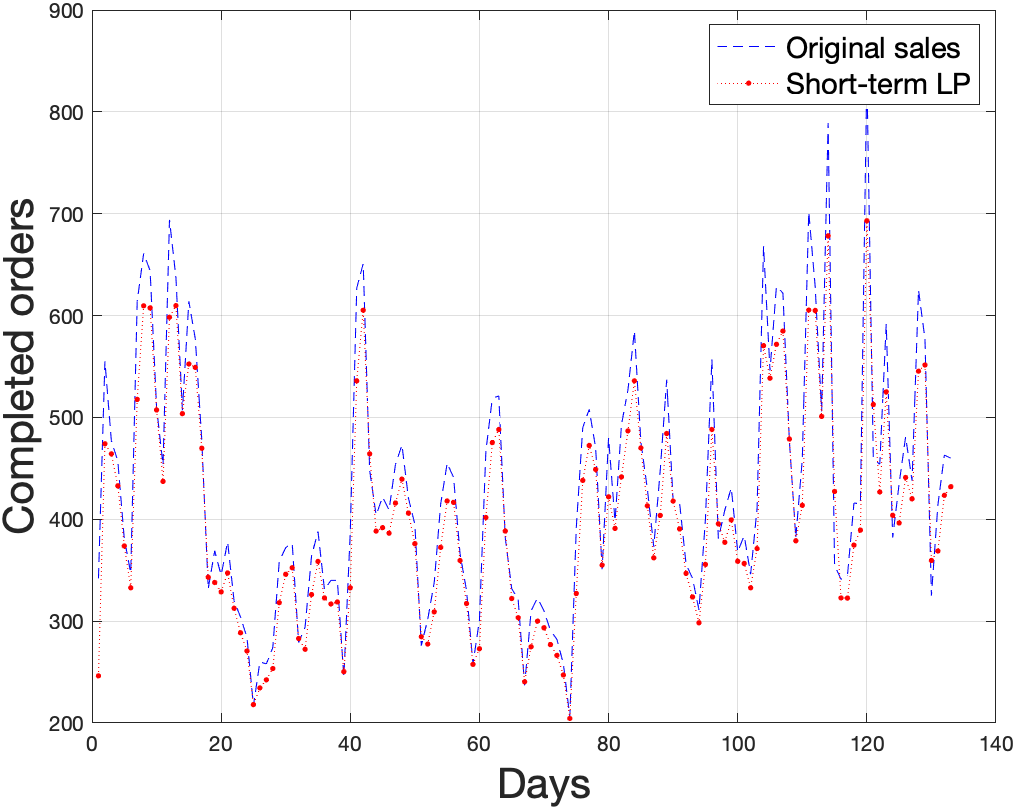
\includegraphics[width=\textwidth]{figures/expLP.png}
            \caption{Standard LP.}
            \label{fig:slpres}
        \end{subfigure}
        \hspace{0.1\textwidth}
        \begin{subfigure}[b]{0.4\textwidth}
            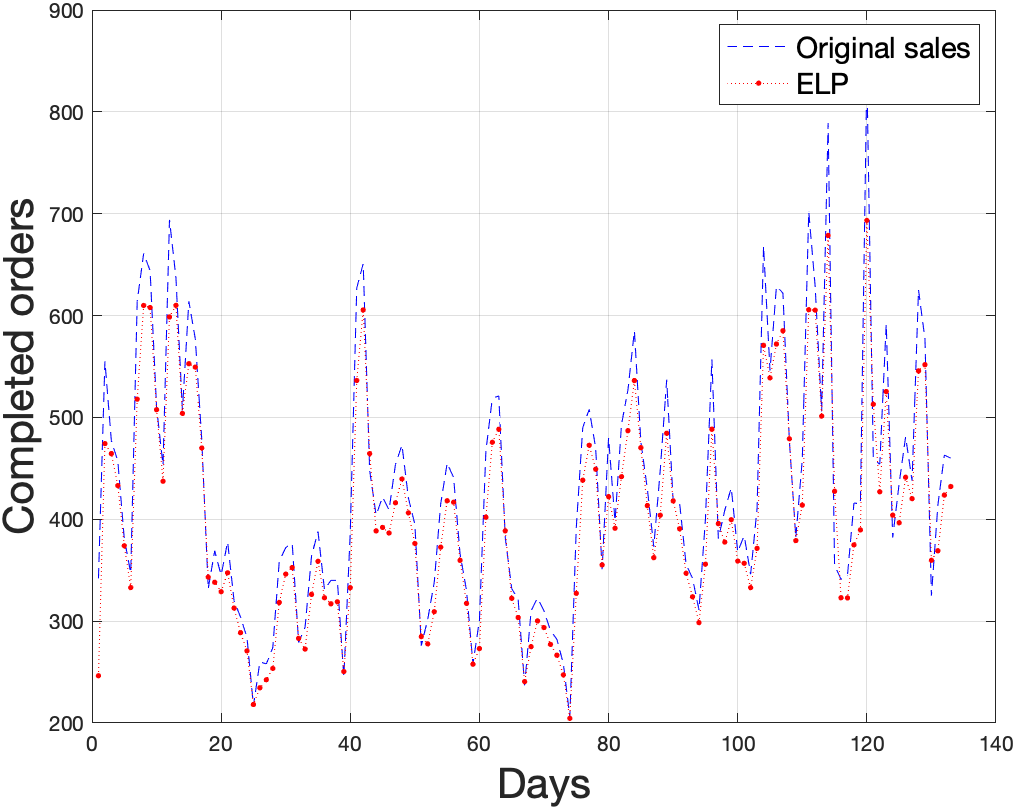
\includegraphics[width=\textwidth]{figures/expELP.png}
            \caption{Extended LP.}
            \label{fig:slpmse}
        \end{subfigure}
        \caption{Results of shot-term linear prediction.}
        \label{fig:shortresult}
    \end{figure}
    
    \subsubsection{Long-term linear prediction} \label{subsec:res_ltlp}
    ~an~R² value of 0.9160 means that 91.6\% of the~variation in the~dependent
    variable can be explained by the~independent variables in the~model.\\
    \\
    RMSE (Root Mean Square Error) and MSE (Mean Squared Error) are measures of the
    error or difference between the~actual values of the~dependent variable and the
    predicted values from the~model. RMSE is the~square root of the~average squared
    difference between the~predicted and actual values, while MSE is simply the
    average squared difference between them.\\
    \\
    In this case,~an~RMSE of 35.0163 means that on average, the~predicted values from
     the~model are about 35.02 units away from the~actual values. And the
    MSE of 1223.3 means that on average, the~squared difference between the~predicted
    and actual values is 1223.3. On figure \ref{fig:longresult} we can see predicted
    orders and on figure \ref{fig:ltlpmse} is the~prediction error for short-term
    linear prediction.
    \begin{figure}[h!]
        \centering
        \begin{subfigure}[b]{0.4\textwidth}
            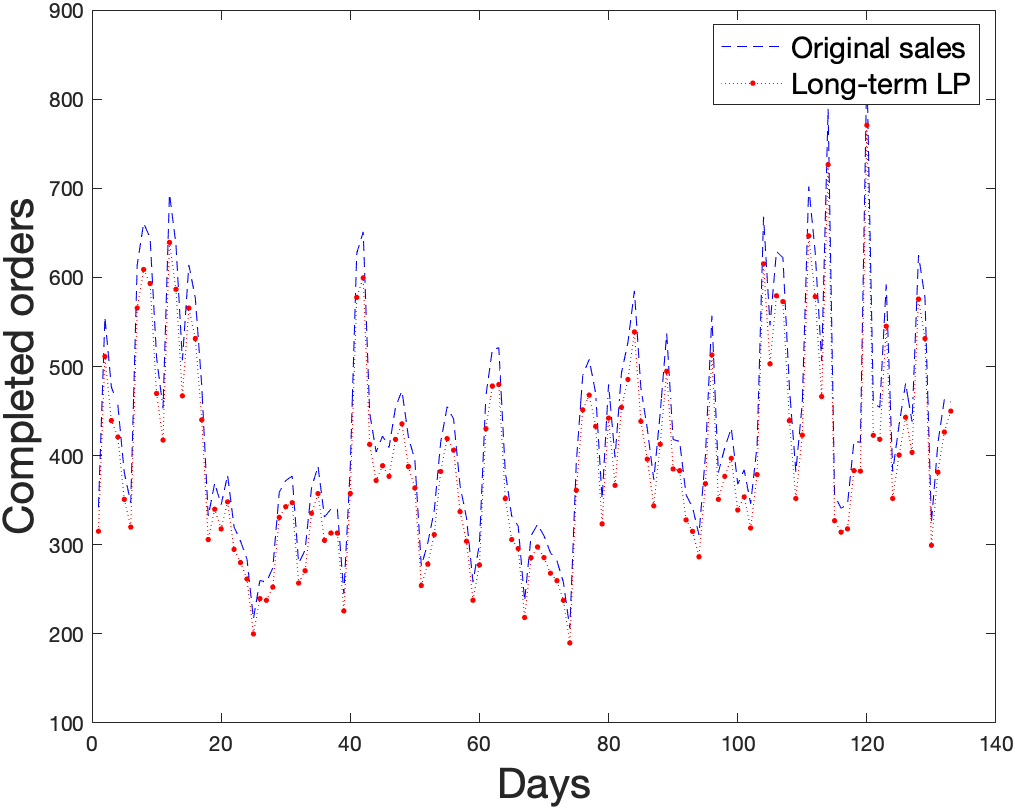
\includegraphics[width=1\textwidth]{figures/expLTLP.png}
            \caption{Standard LP.}
            \label{fig:ltlp}
        \end{subfigure}
        \hspace{0.1\textwidth}
        \begin{subfigure}[b]{0.4\textwidth}
            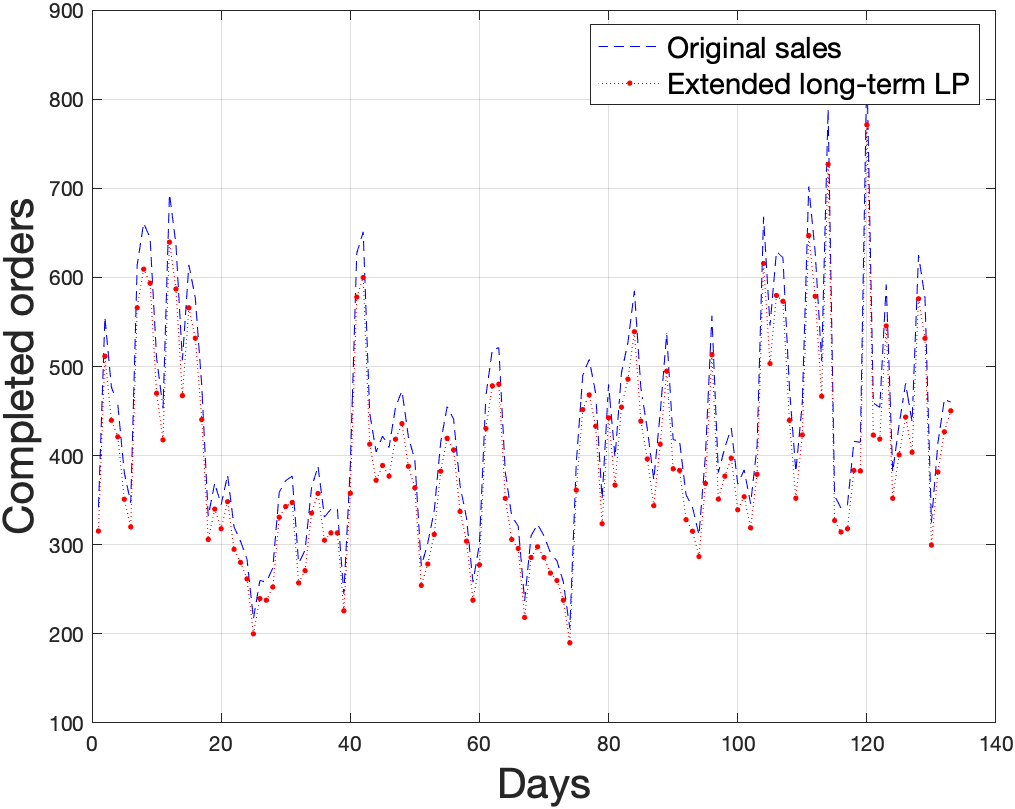
\includegraphics[width=1\textwidth]{figures/expELTLP.png}
            \caption{Extended LP.}
            \label{fig:eltlp}
        \end{subfigure}
        \caption{Results of long-term linear prediction.}
        \label{fig:longresult}
    \end{figure}
    
    \subsubsection{Extended long-term linear prediction} \label{subsec:res_eltlp}
     the~R-squared value of 0.9171 indicates that the~independent variables in the
    model can explain about 91.7\% of the~variation observed in the~dependent variable.
     the~RMSE and MSE are metrics used to evaluate the~accuracy of the~model's predictions
    compared to the~actual values. The~RMSE value of 34.7782 means that the~average difference
    between the~predicted and actual values is approximately 34.7 units. The~MSE value of
    1206.7 indicates that the~average squared difference between the~predicted and actual
    values is approximately 1206.7.\\
    \begin{figure}[!ht]
        \centering
        \begin{subfigure}[b]{0.4\textwidth}
            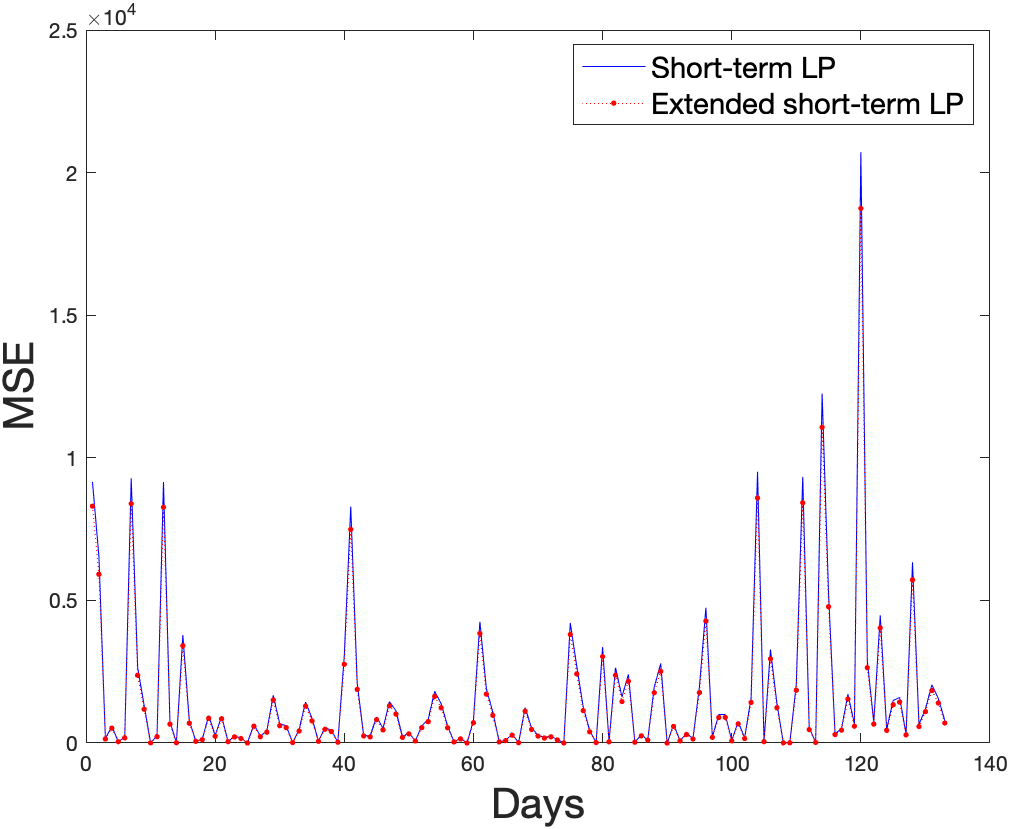
\includegraphics[width=1\textwidth]{figures/mseLP.png}
            \caption{Short-term LP.}
            \label{fig:mselp}
        \end{subfigure}
        \hspace{0.1\textwidth}
        \begin{subfigure}[b]{0.4\textwidth}
            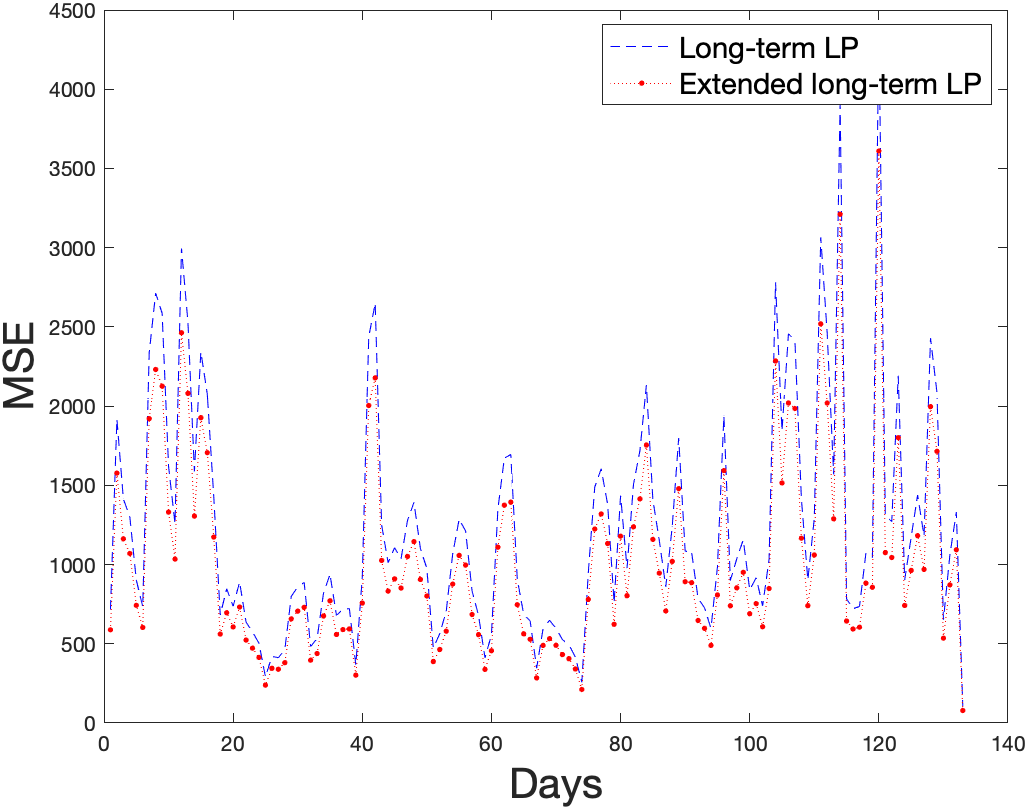
\includegraphics[width=1\textwidth]{figures/mseLLP.png}
            \caption{Long-term LP.}
            \label{fig:ltlpmse}
        \end{subfigure}
        \caption{Comparison of MSE for standard and extended LP.}
        \label{fig:mseresult}
    \end{figure}
    Overall, higher R-squared values and lower RMSE and MSE values in this model are
    desirable as they indicate a~better fit of the~model to the~data and better predictive accuracy.
    
    \subsubsection{Comparison of the~predictors} \label{subsec:res_comparison}
    Let's see results from our experiment in table \ref{tab:model_comparison} as we expected
    long term prediction is worst than long term prediction and apply extended weights to
    linear prediction made all comparison parameters better.\\
    \\
    On the~figures with MSE representation we can see the~main better point of long-term
    prediction for economical datasets. From $R^2$ and RMSE the~improvments of the~models is not
    see so higher than on the~figure \ref{fig:mseresults}.\\
    \newpage
    \begin{table}[!ht]
        \centering
        \begin{tabular}{|l|c|c|c|}
            \hline
            Model & $R^2$ & RMSE & MSE \\
            \hline
            Short-term linear prediction & 0.8872 & 40.6215 & 1650.1 \\
            Extended short-term linear prediction & 0.8881 & 40.4662 & 1637.5 \\
            Long-term linear prediction & 0.9160 & 35.0163 & 1223.3 \\
            Extended Long-term linear prediction & 0.9171 & 34.7782 & 1206.7 \\
            \hline
        \end{tabular}
        \caption{Comparison of linear prediction models}
        \label{tab:model_comparison}
    \end{table}

    \begin{figure}[h!]
        \centering
        \begin{subfigure}[b]{0.4\textwidth}
            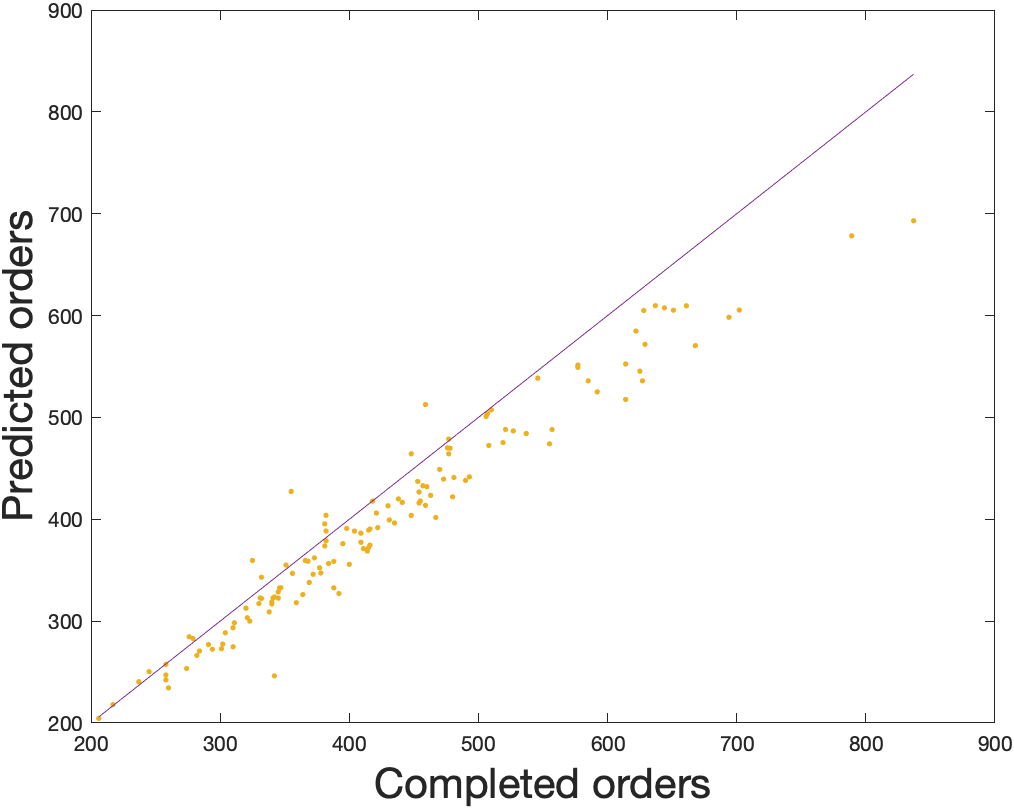
\includegraphics[width=\textwidth]{figures/expCompLP.png}
            \caption{Short-term linear prediction.}
            \label{fig:stlpres}
        \end{subfigure}
        \hspace{0.1\textwidth}
        \begin{subfigure}[b]{0.4\textwidth}
            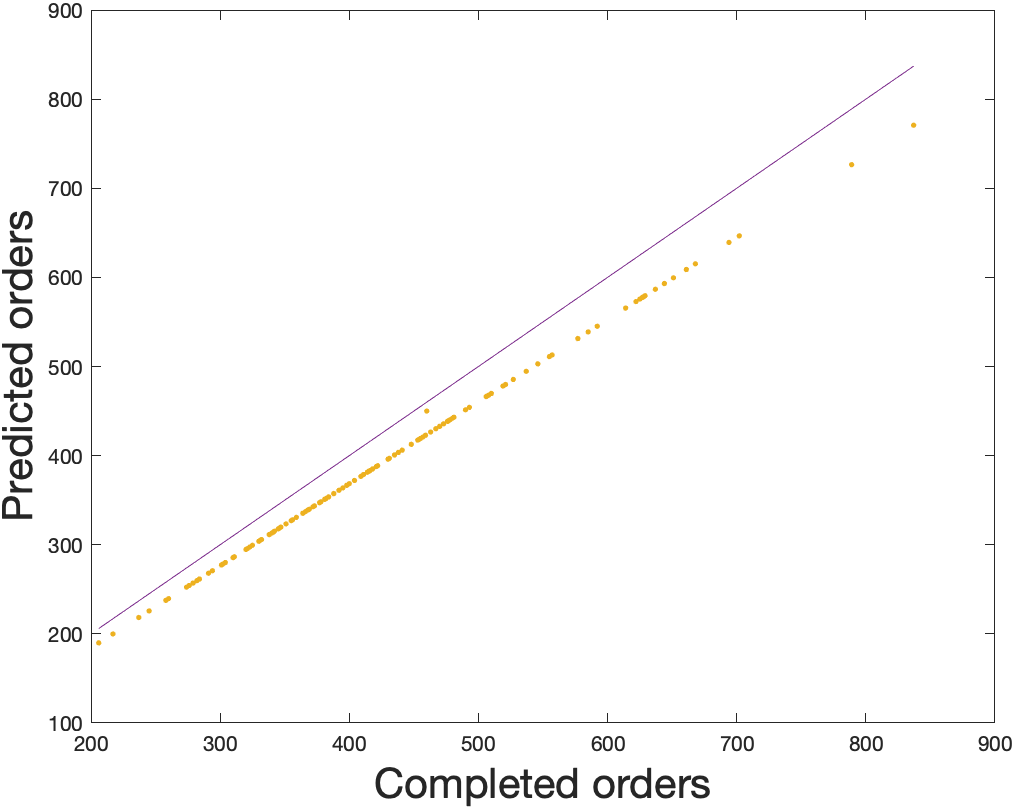
\includegraphics[width=\textwidth]{figures/expCompLTLP.png}
            \caption{Long-term linear prediction.}
            \label{fig:eltlpres}
        \end{subfigure}
        \begin{subfigure}[b]{0.4\textwidth}
            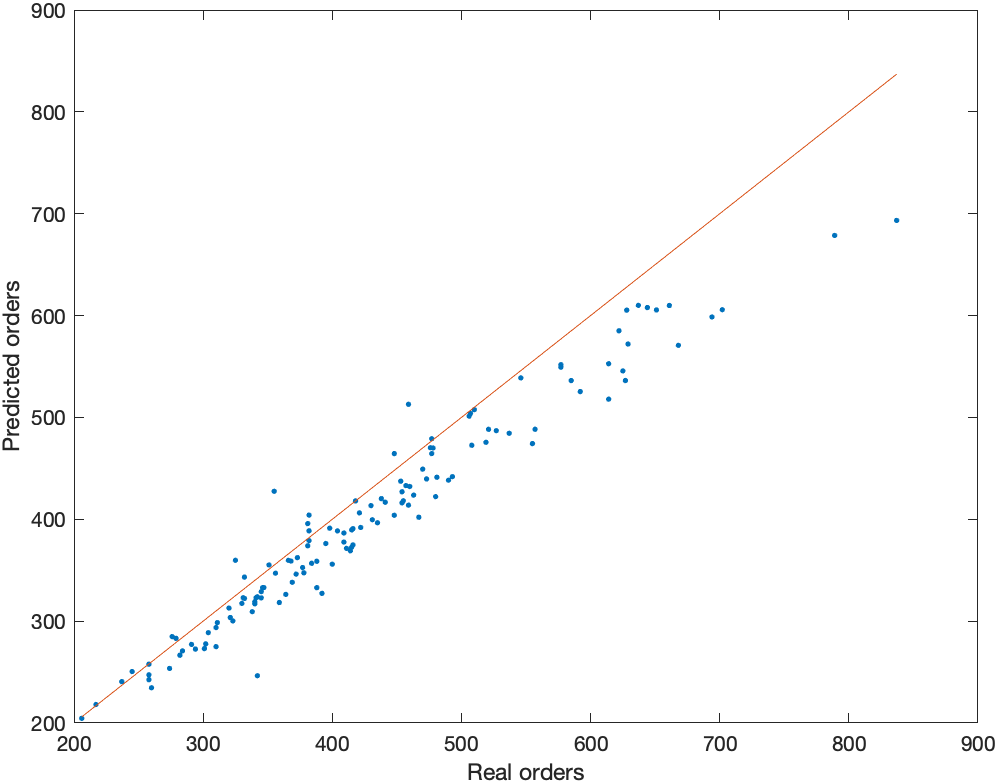
\includegraphics[width=\textwidth]{figures/expCompELP.png}
            \caption{Extended short-term LP.}
            \label{fig:eslpmse}
        \end{subfigure}
        \hspace{0.1\textwidth}
        \begin{subfigure}[b]{0.4\textwidth}
            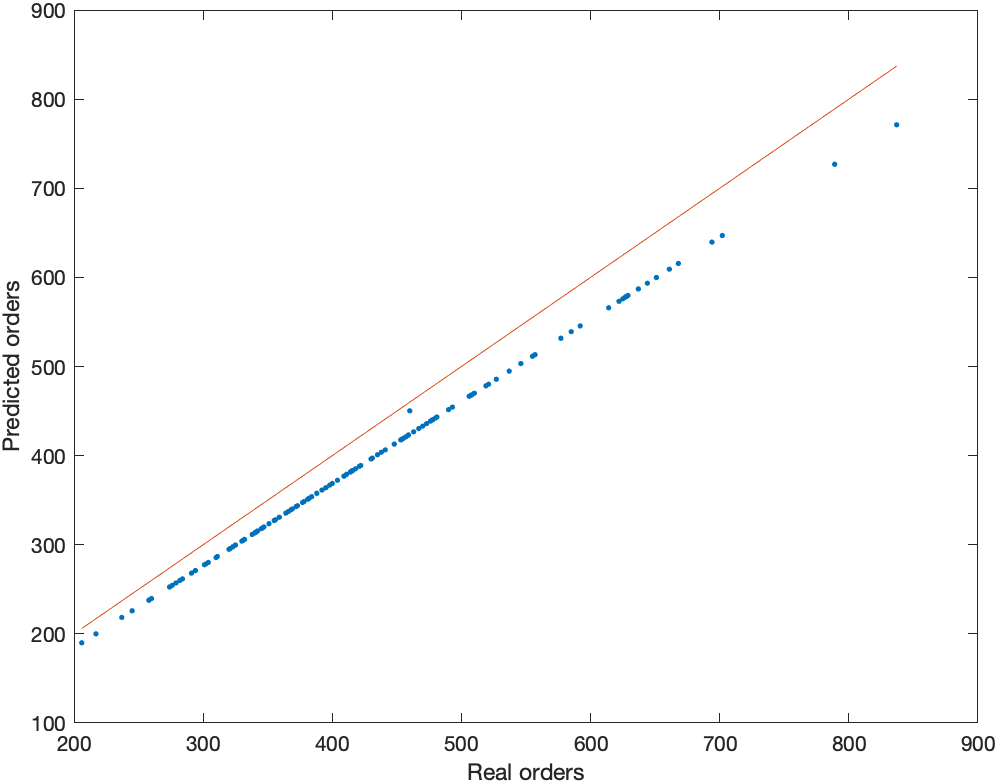
\includegraphics[width=\textwidth]{figures/expCompELTLP.png}
            \caption{Extended long-term LP.}
            \label{fig:eltlpmse}
        \end{subfigure}
        \caption{Results of prediction success.}
        \label{fig:mseresults}
    \end{figure}
    
    On the figure~\ref{fig:mseresults} we can see the main results and
    differences between the models. We can see the less variance in
    long-term predictors (figures \ref{fig:eltlpres}, \ref{fig:eltlpmse})
    than in short one (figures \ref{fig:stlpres}, \ref{fig:eslpmse}).

% !TEX root = ../thesis.tex

\chapter{Summary} \label{summary}

% good linebraking of bibtex url
\setcounter{biburllcpenalty}{7000}
\setcounter{biburlucpenalty}{8000}

%% The bibliography
\printbibliography[heading=bibintoc]

\label{theend} % the last page of the thesis

% List of acronyms
\printglossary[type=\acronymtype,title={\acrlistname}]

% Glossaries
\printglossary

%% Appendix
% !TEX root = ../thesis.tex

\chapter*{\appendixlistname}
\addcontentsline{toc}{chapter}{\appendixlistname}

\begin{description}
    \item[\appendixname{} A] Flowcharts
\end{description}

\appendix
\renewcommand\chaptername{\appendixname}
% !TEX root = ../thesis.tex

\chapter{Flowcharts}

\section{Short-term linear prediction}

\section{Long-term linear prediction}

\section{Extended long-term linear prediction}


% zivotopis autora
%\curriculumvitae\protect
%Táto časť\/ je nepovinná. Autor tu môže uviesť\/ svoje biografické
%údaje, údaje o~záujmoch, účasti na~projektoch, účasti na~súťažiach,
%získané ocenenia, zahraničné pobyty na~praxi, domácu prax, publikácie
%a~pod.

\end{document}
